\documentclass{aicom2e}
\usepackage{amsmath}
\interdisplaylinepenalty=2500
\usepackage[algo2e,ruled,vlined,linesnumbered]{algorithm2e}
\usepackage[active]{srcltx}


\usepackage{amsthm, amssymb,amsfonts}
\usepackage{graphicx}
\usepackage{epsfig}
\usepackage{latexsym}
\usepackage{colortbl}
\usepackage{times}
\usepackage{helvet}
\usepackage{courier}
\usepackage{caption}
\usepackage{subfig}
\usepackage{float}
\usepackage{xcolor}
\usepackage{pslatex}
\usepackage{eso-pic}
\usepackage[bottom]{footmisc}
\usepackage{url}
\usepackage{etex}


\newtheorem{definition}{Definition}
\newtheorem{lemma}{Lemma}
\newtheorem{corollary}{Corollary}

\newtheorem{theorem}{Theorem}
\newtheorem{observation}{Observation}
%\newcommand{\kgs}{$k$-goal problem}
\newcommand{\kgs}{$k$GP}
\newcommand{\kgbfs}{$k$-goal best-first search}


\newcommand{\astar}{A$^*$}
\newcommand{\kastar}{kA$^*$}
\newcommand{\kastarmin}{kA$^*_{min}$}
\newcommand{\kastarmax}{kA$^*_{max}$}
\newcommand{\kxastar}{k$\times$A$^*$}
\newcommand{\astari}[1]{A$^*_#1$}

\newcommand{\minf}{$F_{min}(n)$}
\newcommand{\maxf}{$F_{max}(n)$}
\newcommand{\tuple}[1]{\ensuremath{\left \langle #1 \right \rangle }}
\newcommand{\open}{\textsc{Open}}
\newcommand{\closed}{\textsc{Closed}}
\DeclareMathOperator*{\argmin}{\arg\!\min}
\newcommand{\roni}[1]{\textbf{[RS:#1]}}
%\newenvironment{proof}{\noindent{\bf Proof:~~}}{\qed}

\begin{document}
\begin{frontmatter}                           % The preamble begins here.
%
%\pretitle{Pretitle}
\title{Shortest Path for K Goals}
% \runningtitle{Running title}
%\subtitle{Subtitle}
\maketitle
%
\author[]{Ariel Felner}
\address{Ben Gurion University of the Negev\\ Be'er Sheva, Israel\\
    E-mail: felner@bgu.ac.il}

\author[]{Meir Goldenberg}
\address{The Jerusalem College of Technology\\ Jerusalem, Israel\\
    E-mail: mgoldenbe@gmail.com}
\author[]{Roni Stern}
\address{Ben Gurion University of the Negev\\ Be'er Sheva, Israel\\
    E-mail: roni.stern@gmail.com}

\begin{abstract}
Abstract...

\end{abstract}

\begin{keyword}
artificial intelligence\sep AI\sep Heuristic Search
\end{keyword}
%
\end{frontmatter}

\section{Introduction}

% SPP is classical, important and super general

The shortest path problem (SPP) in a graph is a fundamental problem in Computer
Science, with many applications in Artificial Intelligence and Operations
Research. The input to an SPP problem is a graph and two vertices -- a {\em
start} vertex and a {\em goal} vertex -- and the task is to find the
lowest-cost path in the graph from start to goal. Classical algorithms such as
Dijkstra's algorithm~\cite{DIJ59} and \astar{}~\cite{hartNR68Astar} have been
proposed for solving SPP. SPP algorithms have been applied to various types of
graphs. In some cases, the graph is given explicitly, e.g., representing
roadmaps, grids and game maps~\cite{sturtevant2012benchmarks}. In other cases,
the graph is defined implicitly by an initial vertex and a set of transition
functions, e.g., representing a space of possible robot configurations, puzzle
permutations, or STRIPS-like states in a domain-independent planning problem. 
[[AF: do we want references?]]\roni{Sure, any ideas what to add here?}


% We talk about k SPP

This paper addresses a generalization of SPP, where the task is to solve $k$
SPP problems, such that all the problems share the same start vertex. That is,
we have a single start state and $k$ goal states, and the task is to find $k$
shortest paths, where each path is a shortest path from the start state to a
different goal state. We denote this problem as the {\em $k$-goal} problem
(\kgs{}).


% k-goal is not TSP

\kgs{} is similar but different from previously studied tasks such as the
traveling saleman problem (TSP) and incremental
search~\cite{koenig2004lifelong}. In TSP, the task is to find a single path
that passes through a set of vertices. By contrast, in \kgs{} we aim for $k$
paths, one per goal. In incremental search we have a single goal but the
underlying graph changes. By contrast, in \kgs{} the underlying graph is static, 
but we are given $k$ goals upfront. % and the task is to find paths for all these goals.


% Motivation 1. Star-shaped tour

\kgs{} has many applications. Assume a tour planning application. It is common
to prefer staying in the same hotel when visiting a city, visiting different
sites in different days but returning every night to the same hotel to avoid
packing and unpacking. Path planning under this constraint is thus a \kgs{}
instance, as we have a single common start state and multiple goal states.

% Motivation 2. Choosing between multiple sites

A related example for \kgs{} occurs when planning a family vacation. Assume
that there are $k$ amusement parks and the family wishes to stop in one of
them. It is hard, or even impossible, to exactly model the preferences of the
different family members, but clearly the cost of getting to each of the
different amusement parks is an important consideration for the family members
to know about. Here too, we have a \kgs{} problem, where the start state is the
family's home and the goals are the different amusement park. This represents a
more general scenario that occurs when developing an intelligent personal
assistant, where the planning component may be decoupled from the agent's
high-level decision making component, e.g. when following a
Believe-Desire-Intention (BDI)
architecture~\cite{bratman1999intention,georgeff1998belief}. In such cases
there may be multiple goals an agent may wish to achieve and the cost of
reaching them is important input to the agent's decision making module.


Efficient solutions to the $k$-goal problem can be helpful in many robotic
challenges. For example, consider the task of deploying multiple drones from a
a central dispatcher location to $k$ locations. Another robotic application
where the search for $k$ goals is needed is when using the Incremental Roadmap
Spanner technique~\cite{marble2013asymptotically}, which is a motion planning
technique that includes searching for the shortest path to a limited number of
nearby locations. In fact, preliminary work on using heuristic search to solve
\kgs{} was done exactly for this problem~\cite{DobsonB14}. [[AF: state exactly
which of our versions they used. For example, say: they used a variant of the
KMIN algorithm presented below.]]\roni{We can't say that here because we did not introduce our algorithms. 
But it is good to say that later TODO}

A trivial solution to \kgs\ is to independently run a SSP solver $k$ times. We
analyze the runtime of this option and identify potential redundancies. Then,
we propose an alternative approach where a single search algorithm is used to
search for a vector of $k$ goals, avoiding some of these redundancies. We refer
to this framework as \kastar{}. Implementing \kastar{} includes several design
choices, such as how to aggregate multiple heuristic estimates and what to do
after an optimal path to one of the goals is found. We analyze the theoretical
properties of these different design choices and point out their pros and cons.
Then, we provide a theoretical and experimental study that compare the
\kastar{} approach and the simpler, independent $k$ searches approach,
providing useful guidelines for when to use which option.

%\roni{We need to think about the term {\em concurrent} in our context. I fear it will seem that we are talking about parallel computation.}
%\roni{TODO: SOME RELATED WORK? AF: which one?}

\section{Background and Problem Definition}

%In this section, we formally define the $k$-goal search problem.

% Graphs, costs, SSP

Let $G=(V,E,w)$ be a weighted graph, where $V$ is the set of vertices, $E$ is
the set of edges, and $w:E\rightarrow \mathbb{R}^+$ is a function that assigns
a non-negative real value to each edge. This value is referred to as the {\em
cost} of the edge. The cost of a path in a graph is the sum the edge costs
along it. In the Artificial Intelligence literature, graphs are often used to
represent state spaces, where the graph vertices represent possible states of
the world, the out-going edges of a vertex represent possible actions that an
agent can perform at the corresponding state, and the cost of an edge
represents the cost of the corresponding action. Thus, throughout this paper we
will use the terms {\em states} and {\em actions} instead of vertices and
edges, respectively, and use the term {\em applying an action} instead of
traversing an edge. Note that a path in a graph corresponds to an applicable
sequence of actions.

\begin{definition}[The Shortest Path Problem (SPP)]
A shortest path problem (SPP) is defined by a tuple $\tuple{G,s,g}$, where $s$
and $g$ are states in $G$ and the problem is to find the lowest cost path in
$G$ from $s$ to $g$. \label{def:spp}
\end{definition}

\subsection{The \astar{} Algorithm}




\begin{algorithm2e}[t!]
    \small
    \KwIn{Start state $s$, Goal state $g$)}
    $g(s)\gets 0$; \open{}~$\gets\emptyset$; \closed{}~$\gets \emptyset$\\
    Add $s$ to \open{} with key $f(s)=g(s)+h(s)$\\
    \While {\open{} $\neq \emptyset$} {
        $best \gets $ a state from \open{} with the smallest key \nllabel{line:open:chooseNode}\\
        Move $best$ from \open{} to \closed{}\\
        \lIf {$best$ is the goal}{\Return the best path found to $best$}
        \For{every action $A$ applicable at state $best$ \nllabel{line:nextNeighbor}}{
            $c \gets $ generate a state by applying $A$ to $best$ \nllabel{line:astar:generate-start}\\
            $g_{new}\gets g(best)+w((best,c))$\\
            % Duplicate detection
            \If{$c$ in $\open{}\cup \closed{}$ \nllabel{line:dd-start}}{
                \If{$g(c) \leq g_{new}$}{
                    {\bf continue} (goto line~\ref{line:nextNeighbor})
                }
                Remove $c$ from \open{} and \closed{}  \nllabel{line:dd-end}\\
            }
            % Update n's g and f values
            $g(c)\gets g_{new}$ \nllabel{line:compute-f}\\
            Add $c$ to \open{} with key $f(c)=g(c)+h(c)$  \nllabel{line:astar:generate-end}\\
        }
    }
    \Return No solution exists\\
    \caption{\astar{}}
    \label{alg:astar}
\end{algorithm2e}



% A* for single agent search
SPP has been well-studied in the literature. \astar{}~\cite{hartNR68Astar} is a popular
 heuristic search algorithm for solving SPP. For completeness, we provide a short description of \astar{}
 and provide its pseudo code in Algorithm~\ref{alg:astar}. \astar{} maintains two lists of states: \open{} and
\closed{}. Initially, \closed{} is empty and \open{} contains only the start
state ($s$). Every state that is added to \open{} is associated with a $g$
value and an $f$ value. The $g$ value of a state $n$, denoted $g(n)$, is the
cost of the lowest cost path found so far from the start state $s$ to $n$.
Hence, $g(s)$ is set to zero.
The $f$ value of $n$, denoted $f(n)$, is the sum
of $g(n)$ and a heuristic estimate of the cost of the lowest cost
path from $n$ to the goal state $g$. This heuristic estimate is denoted
by $h(n)$. %, and there is an abundance of prior work in the literature on how to develop heuristics that

[[AF: In all our previous paper we always used $g$-value and $f$-value etc.
Please change to this notation unless you really do not want to]]\roni{I really do not want to}

In every iteration of \astar{}, the state with the lowest $f$ value in \open{}
is moved from \open{} to \closed{}. If that state is a goal, the search halts
returning the path found to it.\footnote{We omit in this pseudo code how
back-pointers are maintained to  preserve the best path to each state.}
Otherwise, the state is {\em expanded}. Expanding a state $n$ means generating
every state that can be reached by applying a single action at state $n$. Then,
the $g$ and $f$ values of every generated state $c$ are computed based on the
$g$ value of its parent, the cost of the action used to generate $c$, and the
heuristic estimate $h(c)$. Finally, the generated states are added to \open{}
with their $f$ values, to be considered for expansion in future iterations. If
the searched graph is not a tree, multiple paths to the same state may be
explored. To address this, \astar{} keeps track of the states it has generated
and maintains for every state only the best (lowest cost) path found to it (lines~\ref{line:dd-start}-\ref{line:dd-end}).


%\roni{TODO: Maybe add more line numbers to the text?} \roni{TODO: Add something on tie breaking [[AF: do not do any of these]]}






% A* properties and admissible heursitics

\astar{} has several important properties. First, if the heuristic used is {\em
admissible}, i.e., it does not over-estimate the cost of the lowest cost path
to the goal, then \astar{} is guaranteed to solve SPP, i.e., to return a lowest
cost path from $s$ to $g$.\footnote{In fact, it is sufficient that the
heuristic is admissible only for the states that are on a single lowest-cost
path for \astar{} to guarantee
optimality~\cite{karpas2012optimal,dechter1985generalizedBestFirst}.} Second,
if the heuristic is {\em consistent} then \astar{} is guaranteed to never
expand a state more than once.
%when a state $n$ is expanded it is guaranteed that the lowest cost path from $s$ to $n$ has been found, and thus $g(n)$ is the cost lowest cost path from $s$ to $n$.
\begin{definition}[Consistent Heuristic~\cite{hartNR68Astar}]
    A heuristic $h$ is {\bf consistent} if for every pair of states $x$ and $y$
    it holds that $h(x)\leq d(x,y)+h(y)$, where $d(x, y)$ is
    the cost of the lowest-cost path from $x$ to $y$.
    \label{def:consistent}
\end{definition}



%The important implication of a consistent heuristic is that \astar{} with a consistent heuristic is guaranteed to expand every state at most once.

Third, under some conditions, it can be shown that up to tie-breaking between
states with equal $f$ values, \astar{} will only expand the minimal set of
states required to find an optimal
solution~\cite{dechter1985generalizedBestFirst}. A recent variant of \astar{}
provides a similar guarantee with respect to the number of states generated as
well~\cite{goldenberg2014enhanced}. This type of guarantees, often referred to
as the {\em optimally effective} property of \astar{}, is  important because in
many cases the runtime of the algorithm is correlated with the number of states
expanded/generated. Thus, guaranteeing that \astar{} expands/generates the
minimal number of states provides some sort of optimality guarantee for
\astar{}'s efficiency compared to other equally informed algorithms.

%[[AF: not sure what is the point in the last sentence. In fact, the A* section can be significantly squeezed.]]\roni{1. I don't see a reason to squeeze the \astar{} section. This paper addresses a simple enough topic that it should be easily accessible to non-search people as well. 2. The last sentence aims to say that \astar{} is optimally effective and why this is important but without committing to the exact details of optimality}

\subsection{The $k$-Goal Problem}

In this paper we focus on the $k$-goal search problem, which can be viewed as
a generalization of SPP.

%\begin{definition}[$k$-goal search]
%   A \kgs\ problem is defined by a tuple $\tuple{G,s, g_1, g_2, \ldots, g_k}$,
%   where $s$ and $g_1, g_2, \ldots, g_k$ are states in $G$ and the problem is to find
%   $k$ paths $p_1,\ldots p_k$ such that for every $i\in [1,k]$ it holds that $p_i$ is a lowest-cost path from $s$ to $g_i$.
%   \label{def:k-goal}
%\end{definition}


\begin{definition}[$k$-goal problem]
A \kgs\ problem is defined by a tuple $\tuple{G,s, \textbf{g}}$ where $G$ is a
graph $s$ is state in $G$, and $\textbf{g}=(g_1,g_2,\ldots,g_k)$ is a vector of
$k$ states. A solution to the \kgs{} problem is a vector of $k$ paths
$\textbf{p}=(p_1,\ldots p_k)$ such that for every  $i\in [1,k]$ it holds that
$p_i$ is a lowest-cost path from $s$ to $g_i$. \label{def:k-goal}
\end{definition}


% k searches independentaly

[[AF: I do not like your notation for vectors. I prefer overline. Your call]]
\roni{I saw both in many papers. But mostly I saw the bold notation (although I am used to the overline from school). Keeping it as is.}

Clearly, SPP is a special case of \kgs\ with $k=1$. A trivial solution to \kgs\
is to consider it as $k$ independent SPPs and use \astar{} (or any other SPP
algorithm) multiple times to solve these $k$ problems. In the next section we
present this approach and analyze its complexity. In later sections we
introduce a different approach that activates a single search that aims to find
all $k$ goals concurrently. This allows sharing and re-using information
between the $k$ different tasks, potentially decreasing the overall search
effort.


\section{$k$ Independent Searches}
\label{sec:k-one-goal}
\begin{algorithm2e}[t!]
    \small
    \KwIn{Start state $s$, Goals vector $\textbf{g}=(g_1,\ldots g_k$)}
    \For{$i$=1 to $k$}{
        $p_i\gets$ \astar{}($s$,$g_i$)\\
    }
    \Return $p_1,\ldots p_k$\\
    \caption{\kxastar{}: \kgs{} with $k$ \astar{}s}
    \label{alg:k-searches}
\end{algorithm2e}




Algorithm~\ref{alg:k-searches} outlines the trivial approach for solving
\kgs{}: running \astar{} $k$ times, one for each of the $k$ goals. The
resulting $k$ paths are returned as a solution to the \kgs{} problem. We refer
to Algorithm~\ref{alg:k-searches} as \kxastar{}.


To analyze the effectiveness of \kxastar{}, we use the notions of {\em necessary} states and {\em surplus} states~\cite{goldenberg2014enhanced}.
%\roni{Meir and Ariel: who used this term before us?}

\begin{definition}[Surplus States and Necessary States]
    Let $\Pi$ be a SPP defined by the tuple $\tuple{G,s,g}$, and let $opt_\Pi$ denote the cost of an optimal solution to $\Pi$.
    A state $n$ is called a {\em necessary} state with respect to $\Pi$ if $f(n)<opt_\Pi$.
    A state $n$ is called a {\em surplus} state with respect to $\Pi$ if $f(n)>opt_\Pi$.
\label{def:surplus}
\end{definition}
Without any additional knowledge of the graph $G$, one needs to expand every necessary state in order to solve a given SPP,
and one can solve a given SPP without expanding any surplus state~\cite{dechter1985generalizedBestFirst,goldenberg2014enhanced}.
\astar{} does exactly that: expands all necessary states but never expands any surplus state~\cite{dechter1985generalizedBestFirst}.


Consequently, if $\Pi_i$ is the SPP problem from $s$ to $g_i$
then using \kxastar{} to solve \kgs{} will end up expanding every state that is necessary w.r.t at least one of the $k$ SPP problems $\Pi_1,\ldots \Pi_k$ and never expand any state that is surplus w.r.t all these SPP problems.
Hence, one might think that \kxastar{} is ``optimally effective'' for \kgs{},
expanding exactly the set of needs one must expand in order to solve the problem, up to tie-breaking between states with the same $f$ value.


This conclusion is not accurate, however, as it overlooks two potential sources for improvement:
\begin{itemize}

\item {\bf Learning from experience.}

When solving one of the $k$ SPP problems (e.g., for finding the optimal path for $g_1$),
one gains additional knowledge of the searched graph, which may be used when solving the subsequent
SPPs for the other goals. For example, propagating heuristic values of states between searches to different goals.
%Such knowledge might be propagation of heuristics of states between searches to different goals.

\item {\bf Avoiding expanding a state multiple times.}

The same state can be generated and expanded in multiple SPPs. For example, \kxastar{}
generates the children of the start state at least $k$ times.
This introduces redundancy to the search process that may be avoided.
\end{itemize}

The first source of improvement is related to the literature on incremental
search~\cite{koenig2004lifelong} and to moving-target search
algorithms~\cite{ishida1995moving,koenig2007speeding}. See
Section~\ref{sec:related-work} for details. In this work we focus on the latter
source of improvement. That is, we aim to avoid expanding a state multiple
times when it is needed for finding the lowest cost path to multiple goals.

%in the search process.
%Next, we analyze these redundancies in the search process that are due to such duplicates.

\subsection{Redundancies in the $k$ Independent Searches Approach}


To analyze the redundant operations performed by \kxastar{}, we first describe
the operations performed by \astar{} whenever a state is generated
(lines~\ref{line:astar:generate-start}-\ref{line:astar:generate-end} in
Algorithm~\ref{alg:astar}):

\begin{enumerate}
    \item {\bf Generation}  (lines~\ref{line:astar:generate-start}-\ref{line:dd-end} and \ref{line:astar:generate-end}).
    This refers to computing the generated state by applying an action to the expanded state,
    performing duplicate detection (updating the $g$ value to the generated if needed),
    and inserting the generated state to \open{} (if needed).
    We denote the computational cost of this step as $C_{gen}$.


    \item {\bf Heuristic computation}  (line~\ref{line:compute-f}). This means computing the $h$ value of the generated state.
    We denote the computational cost of this step as $C_{h}$.
\end{enumerate}
The exact value of $C_{gen}$ depends on the domain and various implementation
details, such as the data structure used to implement \open{} and the state
representation. In the textbook implementation of \astar{} on simple domains,
\open{} is implemented as a Binary heap and the domain actions are easy to
compute and so $C_{gen}$ is linear in the size  of a state's representation in
memory and (plus) logarithmic in the size of \open{} (the cost of inserting an
item in a Binary heap). But faster implementations are also possible in some
domains, where adding to \open{} incurs a constant
time~\cite{GILON2016,BurnsHLR12}. Similarly, the cost of the heuristic
computation ($C_h$) can vary widely as well, where some heuristics require
constant time to compute while more sophisticated heuristics may involve
poly-time computations.


%Each of these operations incur some computational cost. Let $C_{gen}, C_{dd}, C_{h},$ and $C_{add}$ denote the average computation cost of the above four operations, generation, duplicate detection, heuristic computation, and insertion into \open{}, respectively. In addition,

%[[AF: either the i is a subscript or in brackets. Standardize.]]
Let \astari{i} denote   the \astar{} search used to solve $\Pi_i$, and let
$Gen(\text{\astari{i}})$ denote the set of states generated by \astari{i}.
Clearly, \kxastar{} incurs at least $\sum_{i=0}^k
|Gen(\text{\astari{i}})|\cdot(C_{gen}+C_{h})$ in terms of computation cost. The
main source of inefficiency is that the intersection between the sets of states
generated by the individual \astar{} searches can be not empty. This indicates
that some states will be generated in more than one of the $k$ searches, 
incurring a cost of $(C_{gen}+C_{h})$ more than once for each of these states.

\begin{figure}
    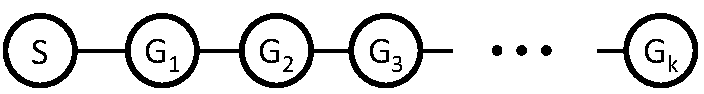
\includegraphics[width=\columnwidth]{k-search-bad_cropped}
    \caption{An example where the $k$ search approach is inefficient.}
    \label{fig:k-search-bad}
\end{figure}
%[[AF: have the goals in the figure be small g not capital]]
An extreme example of this inefficiency is depicted in
Figure~\ref{fig:k-search-bad}. The searched graph is a simple line, where $g_1$ is adjacent to $s$,
$g_2$ is adjacent to $g_1$, and so on. In this case \kxastar{} would generate
$1+2+3+\cdots+k=\frac{k(k-1)}{2}$ states while it is easy to see that
generating $k$ states would be sufficient to solve the \kgs{} for this case.
In the next section we propose an algorithm that attempts to reduce such redundancies. %for solving the \kgs{}  and method for doing so.

% Some costs can be saved

%Some of the costs incurred when generating the same state for more than one goal may be unavoidable. For example, in order to prove that  a path of cost $X$ to a goal $g_i$ is optimal, one needs to expand  all the necessary states w.r.t $\Pi_i$, i.e., generate their children and compute their $f$ values. This is needed to verify that all paths of costs smaller than $X$ have been considered. Since the $f$ value of a state may be different when searching for different goals, this means that a state may be necessary for one search and not necessary for the other.
%Thus, the search must check that $n$ is necessary for each goal independently, incurring a computational cost of $C_{h}$ per goal. However, when a state is generated by more than one search there is potential for saving some of the computational costs incurred during its generation. In particular, by generating such states only once, one may save the costs incurred for state generation ($C_{gen}$).  In the next section we propose a method for doing so.




\begin{table}
	\scriptsize
\begin{tabular}{|m{2cm}|m{5.5cm}|}
        \hline
        \astari{i}  & An \astar{} for finding the lowest cost path to goal $g_i$. \\
        $f(n)$      & The evaluation function used by \astar{}: $f(n)=g(n)+h(n)$ \\
		$F(n)$      & The evaluation function used by \kastar{} \\
		
		%A state evaluation function used by \kastar{} to prioritize \open{}. $F(n)$ aggregates a vector of $k$ possibly different $f$ values to a single value. \\
		\minf{} and \maxf{} & \minf{}=$\min_{j\in[1,k] f(n)}$ and \maxf{}= $\max_{j\in[1,k] f(n)}$\\	
        \kastarmin{} & \kastar{} that uses \minf{} to compute its $F$ values\\		
        \kastarmax{} & \kastar{} that uses \maxf{} to compute its $F$ values\\		
        Gen($X$)    & The set of states generated by algorithm $X$ \\
        Time($X$)   & The runtime required to run algorithm $X$ \\

        \hline
    \end{tabular}
\caption{This table summarizes the notations used in this paper.}
\label{tab:notations}
\end{table}


\section{A Single Search for all  $k$ Goals}
\label{sec:one-k-goal-search}

In this section we generalize \astar{} to search for $k$ goals concurrently. We
call the resulting algorithm \kastar{}. Before presenting a complete pseudo
code for \kastar{}, we highlight several aspects that differentiates it from \astar{}.

\subsubsection*{Multiple heuristics per state.}


When a state $n$ is generated, \kastar{} computes a $k$-ary vector
$\textbf{h}(n)=(h_1(n),\ldots h_k(n))$, where $h_i(n)$ is the heuristic
estimate of the cost to get from $n$ to goal $g_i$. These $k$ heuristic values
are used to form a $k$-ary vector $\textbf{f}(n)=(f_1(n),\ldots f_k(n))$, where
$f_i(n)=g(n)+h_i(n)$. We discuss later how the elements of this $k$-ary vector
of $f$ values are aggregated to a single value denoted $F(n)$ -- which is used
to prioritize
% by taking their minimum or their maximum.
\open. That is, in every iteration \kastar{} selects from \open{} a state with
the lowest $F$ value. Note that the computational effort of generating a state
in \kastar{} is larger than that of regular \astar{}, as it requires computing
$k$ heuristics.

%computing $F$ costs more than computing an individual $f$ value, as it at least $k\cdot C_h$, and thus the computation cost of generating a state in \kastar{} is larger than that of \astar{} by $(k-1)\cdot C_{h}$.\footnote{As discussed later in the paper, the actual computational cost in \kastar{} can be smaller, since as the search progresses the list of relevant goals becomes smaller, and consequently computing $F$ becomes easier.}

\subsubsection*{Maintaining the active goals.}

In \astar{} when a goal is expanded the search halts. By contrast, in \kastar{}
the search does not halt until a lowest-cost path to each of the $k$ goals is
found. To this end, \kastar{} tracks the set of goals for which the lowest-cost
path to them has not been found. This set of goals is referred to as the {\em
active goals}. Maintaining the set of active goals is also used to avoid
redundant heuristic computations: when a state is generated we compute the
heuristics only for goals that are still active.



%\subsubsection*{Node evaluation function.} When searching for a single lowest-cost path with \astar{}, the state are popped from \open{} according to their $f=g+h$ values. In \kastar{}, we compute the $h$-value forand associate every state in \open{} with a value that considers the $h$-value for each of the $k$ goals.     Thus, when a state is generated then we compute the heuristic for each of the $k$ goals.





\begin{algorithm2e}[t!]
    \small
    \KwIn{Start state $s$, goal states $g_1,\ldots,g_k$}
    $g(s)\gets 0$; \open{}~$\gets\emptyset$; \closed{}~$\gets \emptyset$; {\bf p}$\gets \emptyset$\\
    {\color{blue} {\tt ActiveGoals} $\gets \{g_1,\ldots,g_k\}$ \nllabel{line:init-active-goals}} \\
    {\color{blue}$F\gets$ ComputeF(s, ActiveGoals) \nllabel{line:compute-f-start}}\\
    Add $s$ to \open{} with key {\color{blue} $F(s)$}\\
    \While {\open{} $\neq \emptyset$ and {\color{blue}{\tt ActiveGoals} $\neq \emptyset$}} {
        $best \gets$ a state in $\open{}$ with the smallest key \nllabel{kastar:line:open:chooseNode}\\
        Move $best$ from \open{} to \closed{}\\
        {\color{blue}
        \If {$best\in$ {\tt ActiveGoalsls}}{
            Add the path to $best$ to {\bf p} \nllabel{line:storePath}\\
            Remove $best$ from {\tt ActiveGoals} \nllabel{line:removeGoal}
        }}
        \For{every action $A$ applicable at state $best$  \nllabel{kastar:line:nextNeighbor}}{
            $c \gets $ generate a state by applying $A$ to $best$ \\
            $g_{new}\gets g(best)+w((best,c))$\\
            % Duplicate detection
            \If{$c$ in $\open{}\cup \closed{}$ }{
                \If{$g(c) \leq g_{new}$}{
                    {\bf continue} (goto line~\ref{kastar:line:nextNeighbor})\\
                }
                Remove $c$ from \open{} and \closed{} \\
            }
            % Update n's g and f values
            $g(c)\gets g_{new}$ \nllabel{line:compute-f}\\
            {\color{blue} $F\gets$ ComputeF(n, {\tt ActiveGoals}) \nllabel{line:computeF} \\
                Add $c$ to \open{} with key {\color{blue} $F(c)$}  \\
            }
        }
    }
    {\color{blue} \If{{\tt ActiveGoals} $= \emptyset$}{
        \Return {\bf p}\\
    }}
    \Return No solution exists\\
    \caption{\kastar{}}
    \label{alg:kastar}
\end{algorithm2e}



Algorithm~\ref{alg:kastar} shows the pseudo code for \kastar{}.
We highlighted in blue
the differences between the pseudo code of \astar{} (Algorithm~\ref{alg:astar})
and the pseudo code of \kastar{} (Algorithm~\ref{alg:kastar}).
Initially, all goals are inserted into the set of active goals, denoted  {\tt ActiveGoals}
(line~\ref{line:init-active-goals} in Alg.~\ref{alg:kastar}). Every state
$n$ that is added to \open{} is associated with a value $F$ that is
computed by the {\tt ComputeF} function. In every iteration, the state with
the smallest $F$ value is selected and removed from \open{}
(line~\ref{line:open:chooseNode}). If it is a goal then we store the path to it
(line~\ref{line:storePath}). In addition, we remove that goal from the {\tt
ActiveGoals} list, to mark that we are no longer looking for a path to that
goal (line~\ref{line:removeGoal}). When the {\tt ActiveGoals} list is empty, we
halt the search, having found a path to each goal.

It is easy to see that Algorithm~\ref{alg:kastar} is complete and sound, in
the sense that if there are paths to the $k$-goals then they will be found, and the
paths returned by the algorithm are all valid paths to the $k$ goals. The key
question is whether each of these $k$ paths is indeed
an optimal path to its corresponding goal.
As we show next, this depends on how $F$ is computed, as encapsulated in the {\tt
ComputeF} function (lines~\ref{line:compute-f-start} and~\ref{line:computeF}).

[[AF: In line 23, don't you want to return some of the paths if you have
them?]]\roni{I think this will just confuse. The problem is defined for all the $k$ paths.}

\subsection{An Evaluation Function for \kastar{}}

%In \astar{} for a single goal, states are prioritized in \open{} according to the $f=g+h$ value of a state. In contrast, a state in \kastar{} has a vector of $k$ heuristic values $\textbf{h}(n)$ and consequently a vector of $f$ values $\textbf{f}$(n) that contains one $f$ value per goal. Therefore, \kastar{} requires a state evaluation function that aggregates these $f$ values in some way. In Algorithm~\ref{alg:k-goal-bfs} this is encapsulated in the {\tt ComputeF} function. We refer to the value ($F$) returned by this function as the state's $F$ value, and consider the following two options for computing it.
We consider the following two options for computing the $F$ value of a state:
\begin{align}
\text{\minf{}}=&\min_{i\in [1,k]}f_i(n) \\
\text{\maxf{}}=&\max_{i\in [1,k]}f_i(n)
\end{align}
\kastar{} that uses with \minf{} as the state evaluation function ({\tt
ComputeF}) is referred to hereinafter as \kastarmin{}, and similarly \kastar{}
that uses \maxf{} is referred to as \kastarmax{}. Table~\ref{tab:notations}
summarizes the notations used in this paper.


%\subsection{$F_{min}$}

\begin{theorem}[\kastarmin{} is admissible]
If $h$ is an admissible heuristic, then running \kastarmin{} returns $k$ paths
$\pi_1,\ldots, \pi_k$ such that for every $i$ we have that $\pi_i$ is a lowest cost
path from $s$ to $g_i$. \label{the:min-f}
\end{theorem}
 \begin{proof}
To prove this, we show that when a goal state $g_i$ is expanded for the first
time, then $g(g_i)$ is guaranteed to be the cost of the lowest-cost path from
$s$ to $g_i$. By negation, assume that $g_i$ was expanded, but there is
a better path to $g_i$ that has not yet been discovered. Since \kastar{} (and
in particular, \kastarmin), is a best-first search, \open{} has some state $n$
that is on a better path to $g_i$ and has not been expanded yet. That is,
\begin{equation}
g(n)+h_i(n)<g(g_i)
\label{eq:proof-1}
\end{equation}
Since $g_i$ was chosen to be expanded before $n$, it must have a $F_{min}$ value no-larger than $n$, i.e.,
\begin{align}
F_{min}(n) &\geq  F_{min}(g_i) \\
g(n)+\min_{j\in [1,k]}(h_j(n))& \geq  g(g_i)+\min_{j'\in [1,k]}(h_{j'}(g_i))
\end{align}
Since $h_i(g_i)=0$ then
\[ g(n)+\min_{j\in [1,k]}(h_j(n)) \geq  g(g_i) \]
Finally, since $h_i(n)\geq \min_{j\in [1,k]}(h_j(n))$ it holds that
\[ g(n)+h_i(n) \geq  g(g_i) \]
contradicting Equation~\ref{eq:proof-1}.
\end{proof}


%\subsection{$F_{max}$}

\begin{figure}
 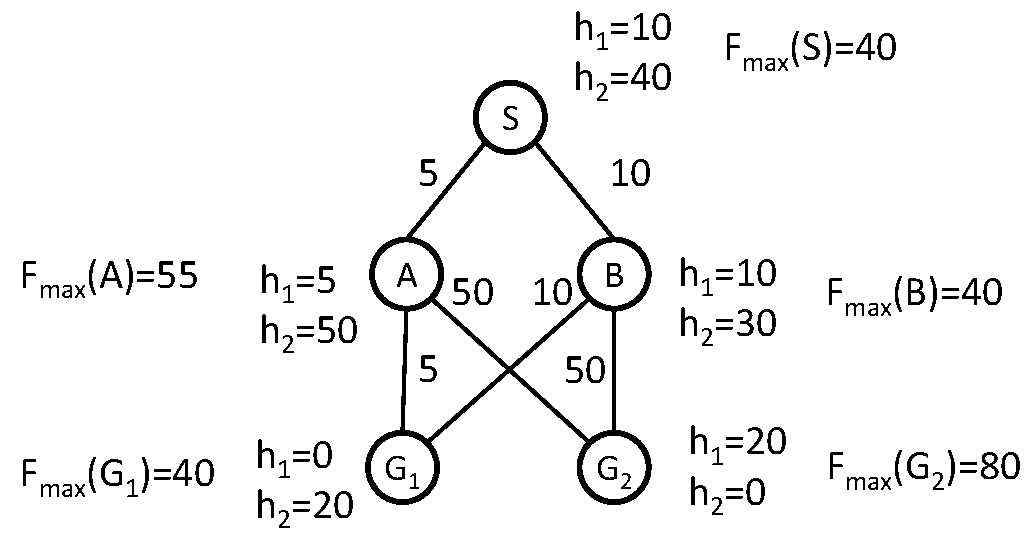
\includegraphics[width=0.85\columnwidth]{max-bad_cropped.pdf}
 \caption{An example of where using \kastarmax{} returns a non-optimal solution. Using \kastarmax{} results in the following expansion order: $S$, $B$, $g_1$.
 Thus, when $g_1$ is expanded, the best path known to it costs 25, while a
 better path to $g_1$ goes through $A$ and costs only 10.}
 \label{fig:max-bad}
 \end{figure}

 \begin{observation}[\kastarmax{} is not admissible]
    Even if $h$ is an admissible heuristic,
    running \kastarmax{} may return a path $\pi_i$ from $s$ to $g_i$ that is not optimal.
    \label{obs:max-f-inadmissible}
 \end{observation}

%[[AF: in the theory above you talked about Fmin and here you talk about kastamx. Use kastarmin too.]]\roni{Maybe you looked at an old version?}

To demonstrate Observation~\ref{obs:max-f-inadmissible}, consider the graph in
Figure~\ref{fig:max-bad}. In this example, using \kastarmax{} results in the
following expansion order: $S$, $B$, and then $g_1$. At this stage, we expanded
one of the goals -- $g_1$ -- while the best path found so far to it goes
through $B$ and costs 40. However, a better path to $g_1$ passes through $A$,
which costs only 10.


 % MAX-F is OK for consistent heuristics


The observant reader may have noticed that the heuristic function in
Figure~\ref{fig:max-bad} is inconsistent (Definition~\ref{def:consistent}):
$h_2(A)=50$ while its child, $g_1$, which is connected to it via an edge of
cost 5, has $h_2(g_1)=20$. If $h$ was consistent then $h_2(A)-c(A,g_1)\leq
h_2(g_1)$, where $c(A,g_1)$ is the cost of the edge between $A$ and $g_1$.
Interestingly, if the heuristic used is consistent then \kastarmax{} is admissible, as proven in the following result. %below. % using \maxf{} is possible [[AF: admissible?]], [[AF: I would only use one term KASTARMAX and never use FMAX. Why do you need both. Your call.]]due to the following result.%n \kastar{} is possible, guaranteeing that all paths returned are optimal.


% wi(Definition~\ref{def:consistent}), then \maxf{} is admissible for \kastar{}. %the inadmissibility of Max-$f$ is related to the {\em inconsistency} of the used heuristic.

% [[AF: the term admissible for k-goals is not fully defined. Let's denote it by k-admissible?]]\roni{I don't think this is needed. Is the text not clear on this?}

\begin{theorem}[\kastarmax{} is admissible if $h$ is consistent]
    If $h$ is consistent, then when
    \kastarmax{} expands a goal state then the optimal path to that goal has been found.
    \label{the:max-f}
\end{theorem}
\begin{proof}
    Let $g^*(n)$ denote the cost of the lowest cost path from $s$ to $n$
    and let $h^*_i(n)$ is the cost of the lowest cost path from $n$ to $g_i$.
    Now, assume that a goal $g_i$ is expanded by \kastarmax{}.
    In \kastar{}, as in \astar{} (and most best-first searches),
    every state $n$ in \open{} represents the best path found so far from the start state to $n$.
    As the search progresses, these paths are extended. % [[AF: extended??]].\roni{Ideas for a better word?}
    Therefore, throughout the search there is always a state $n\in \open{}$
    that is on the optimal path to $g_i$ for which $g(n)=g^*(n)$. This can be proven inductively from the start state. %[[AF: maybe add: this is proved inductively from the start state.]]

    Now, assume by negation that Theorem~\ref{the:max-f} is not correct. This means that
    there is a case where $g_i$ is expanded while $g(g_i)$ is not optimal,
    i.e., $g^*(g_i)<g(g_i)$. Let $n$ be the state in \open{} for which $g(n)=g^*(n)$
    when $g_i$ was expanded. Since the heuristics $h_1,\ldots, h_k$ are all admissible
    then
    \begin{equation}
    g(n)+h_i^*(n) = g^*(n)+h_i^*(n) < g(g_i)
    \label{eq:not-optimal}
    \end{equation}

    Since $g_i$ was chosen for expansion and not $n$, it holds that $ F_{max}(g_i) \leq F_{max}(n) $.
    Following the definition of $F_{max}$, we have that
    \begin{equation}
    g(g_i) + \max_{j\in [1,k]} h_{j}(g_i) \leq g(n)+\max_{j'\in [1,k]} h_j'(n)
    \end{equation}
    %   So, there exists a goal $g_l$ for which $f_l(n)$ is larger than all the $f_j$ values of $g_j$, for all $j\in [1,k]$ ($l$ is t). In particular,
    Let $l=argmax_{j'\in [1,k]} h_{j'}(n)$.
    Then for the goal $g_l$ we have that
    $f_l(g_i) < f_l(n)$ (since $h_l(g_i) \leq \max_{j\in [1,k]} h_{j}(g_i)$), and consequently:
    \begin{align}
    g(g_i)+h_l(g_i) < & g(n)+h_l(n) \\
    g(g_i) < & g(n)+h_l(n) - h_l(g_i)
    \end{align}
    Since we assumed that we have not found the optimal path to $g_i$ (Eq.~ \ref{eq:not-optimal})
    and $g^*(n)=g(n)$ then
    $g(n)+h_i(n)\leq g(g_i)$ and thus:
    \begin{align}
    g(n)+h^*_i(n)  & < g(n)+h_l(n) - h_l(g_i)\\
    \Rightarrow h^*_i(n)  & < h_l(n) - h_l(g_i)\\
    \Rightarrow d(n,g_i) + h_l(g_i) & < h_l(n) \label{eq:h-inconsistent}
    \end{align}
    Thus, Equation~\ref{eq:h-inconsistent} directly contradicts the assumption
    that $h$ is consistent (see Definition~\ref{def:consistent}).
\end{proof}

%[[AF: above you used d(x,y) and here you use c(x,y). Standardize]]

A direct consequence of Theorem~\ref{the:max-f} is that
if the heuristic used by \kastarmax{} is consistent then
it is guaranteed to return an optimal path for all $k$ goals.

\begin{corollary}%[\kastarmax{} is admissible if $h$ is consistent]
%If $G$ is undirected and $h$ is admissible and consistent, then running
If $h$ is admissible and consistent, then running
\kastarmax{} will return $k$ paths $\pi_1,\ldots, \pi_k$ such that $\forall i\in[1,k]$ $\pi_i$ is a lowest cost path from $s$ to $g_i$. \label{cor:max-f}
\end{corollary}

[[AF: I do not like the term maxf and do not like that you say that it is
admissible without exactly defining what you mean. Can you omit this and only
talk on kastarmax]]\roni{Fixed}.

[[ARIEL UP TO HERE]]

\section{Maintaining \open\ in \kastar{}} \label{sec:lazy}


For the rest of this paper we assume that the heuristic $h$ is admissible and
consistent, and thus both \kastar{} versions -- \kastarmax{} and \kastarmin{} -- are valid options. Thus, when a goal $g_i$ is
expanded by \kastar{} (either \kastarmax{} or \kastarmin{}) we are guaranteed that
the optimal path to it has been found. This is why we remove $g_i$ from the
set of active goals (see line~\ref{line:removeGoal} in
Algorithm~\ref{alg:k-goal-bfs}). Removing a goal from the set of active goals
has several potential effects. First, computing the state evaluation function for any state generated from here on will be cheaper, as there is no point in
computing the heuristic function for goals that are no longer active.


\begin{figure}
    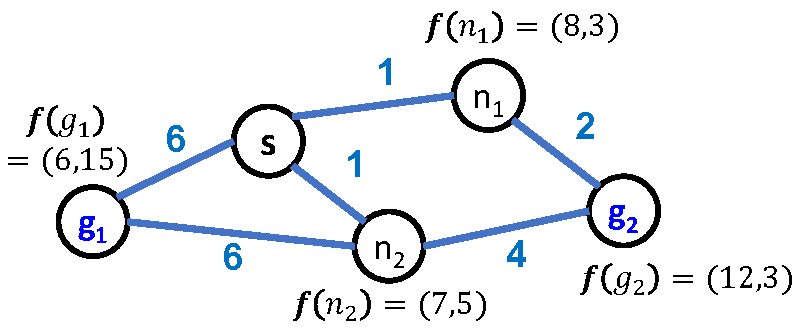
\includegraphics[width=0.7\columnwidth]{need-resort_cropped.pdf}
    \caption{An example where running \kastarmin{} without re-sorting \open{} after a goal is expanded
        results in expanding redundant states ($n_2$).}
    \label{fig:need-resort}
\end{figure}


Second, considering $f$ values for goals that are no longer active provides poor guidance to the search, directing it towards goals that are no longer active. For example, consider the \kgs{} problem depicted in Figure~\ref{fig:need-resort}. Running \kastarmin{} on this instance will result in expanding $n_1$ and then $g_2$. At this stage, \open{} contains $n_2$ and $n_2$ with $F$ values 4 and 5, respectively.
Note that these $F$ values are {\em stale}, in the sense that they
were computed when the active goals included $g_1$ and $g_2$
but now the only active goal is $g_2$.
According to these stale $F$ values, the next state \kastarmin{}
will expand is $n_2$, generating $g_1$ with with a path of at least 7
(since $f_1(n_2)=7$). Note that $n_2$ is a surplus state with respect to both $g_1$ and $g_2$, i.e., expanding it is redundant. Note that re-sorting \open{} after $g_2$ was expanded would have resulted in $n_3$ being expanded before $n_2$ and eventually finding the optimal path to $g_1$ without expanding $n_2$ at all. Thus, some states in \open{} may need to be re-sorted after a goal is expanded.

%The problem is even graver when using \kastarmax{}, where re-computing the $F$ value of some of the states in \open{} is necessary to ensure optimality of the returned paths. For example, consider running \kastarmax{} on the same \kgs{} problem given in Figure~\ref{fig:need-resort}, and assume that all $f$ values are accurate. In this case, $n_2$ will expanded first, followed by $g_2$ and $g_1$ choose from \open{} is $n_1$ with $F(n_1)=5$. and may cause \kastarmin{} to expand states that are surplus for all  for states already generated there is no point in considering the $f$ values for goals that are no longer active, as it will unnecessarily guide the search towards an already achieved goal.







\subsection{Reordering \open\ eagerly}

One option to address this is to completely re-sort \open{} after removing a
goal from the list of active goals (line~\ref{line:removeGoal}). In other
words, when a goal is expanded, recompute the state evaluation function ({\tt
ComputeF}) for all states in \open{} to get an updated $F$ value and then
re-sort \open{} accordingly. We refer to this option as {\em Eager \kastar{}}.






%To quantify the cost of this option, assume without loss of generality that $g_i$ is the  $i^{th}$ goal has been found, and let $Gen_i(\kastar{})$ denote the set of  states generated by \kastar{} until $g_i$ is expanded.


%. Therefore, let $Gen_k(i)$ denote the number of statesgenerated by \kastar{} until the $i^{th}$ goal has been found.\footnote{Notethe $i^{th}$ goal found by \kastar{} is not necessarily goal $g_i$.}

%After the first goal is found, there are $Gen_k(1)$ states in \open{}, and thus re-sorting them will require a computational cost of $Gen_k(1)\cdot (C_{add} + k)$, assuming that re-computing the  evaluation function requires $k$ timesteps -- going over the $k-1$ remaining heuristics and aggregating their values (we assume that every state stores its $h$ values to avoid re-computing them at this stage). After the second goal is found, there are $Gen_k(2)$ state in \open{} but there are fewer heuristics to compute ($k-2$), and thus re-sorting open requires $Gen_k(2)\cdot (C_{add} + k-1)$. Following this reasoning, the extra computational cost incurred by re-sorting after every goal is found is
%\begin{equation}
%\sum_{i=1}^{k-1} Gen_k(i)\cdot (C_{add}+k-i+1)
%\label{eq:re-sort-cost}
%\end{equation}


Eager \kastar{} is a valid option but it can be costly. To quantify the added running time
incurred by Eager \kastar{} when it re-sorts open, we introduce the following notation.
Let $C_r$ the cost of re-computing the $F$ value (using either \minf{} or \maxf{}) for a state and updating its position in \open{} accordingly. Without loss of generality, assume that $g_i$ is the  $i^{th}$ goal has been found, and denote by $Gen_i(\text{\kastar{}})$ the set of  states generated by \kastar{} until $g_i$ is expanded. After the first goal is found, there are at most $|Gen_1(\text{\kastar{}})|$ states in \open{}. Thus, re-sorting them will require a computational cost of at most $|Gen_1(\text{\kastar{}})|\cdot C_r$. After the second goal is found, there
are at most $|Gen_2(\text{\kastar{}})|$ states in \open{} so re-sorting \open{} requires at most
$|Gen_2(\text{\kastar{}})|\cdot C_r$. Following this reasoning, the total computational
cost incurred by Eager \kastar{} for re-sorting \open{} after every goal is found is at most
\begin{equation}
O_{eager}=\sum_{i=1}^{k-1} |Gen_i(\text{\kastar{}})|\cdot C_r
\label{eq:re-sort-cost}
\end{equation}
We denote this extra cost by $O_{eager}$.
An important question is whether $O_{eager}$ is significant with respect to the overall runtime of \kastar{}. Observe that $Gen_k(\text{\kastar{}})$ is the set of all states generated by \kastar{}
and that \kastar{}, and thus the runtime of \kastar{} is at least
$|Gen_k(\text{\kastar{}})|\cdot C_{gen}$.
In addition, note that $C_{gen}$ is larger than $C_r$.
This is because $C_{gen}$ includes the costs of creating the data-structure for representing the generated state and performing duplicate detection,
in addition to the costs of computing the $F$ value and insertion into \open{}.
Thus, if most states were generated when searching for the last goal ($g_k$)
then the extra overhead of Eager \kastar{} is negligible

[[AF: I did not understand the reasoning. Explain me in person]]
\roni{Is it better now?}

\subsection{Partial Resorting of \open{}}
Observe that the $F$ value of some states do not change when re-sorting \open{} after a goal is expanded.
For example, consider a state $n$ with $F$ value that is computed from the vector of $f$ values $\textbf{f}(n)=(10,5,3)$. When using \kastarmin{}, $F(n)=f_3(n)=3$. Therefore, the $F$ value of $n$ will only change if the goal $g_3$ is expanded. Importantly, there is no need to re-compute it after goals $g_1$ or $g_2$ are expanded. More generally, after a goal $g_i$ is expanded there is no need to re-compute the $F$ value
of any state for which $F(n)\neq f_i(n)$.

We implemented this optimization by keeping track of the {\em determining goal} for every state $n$,
that is, the goal $g_i$ for which $F(n)=f_i(n)$. If there are multiple determining goals, we choose one arbitrarily. Then, we only re-compute the $F$ value of a node if its determining goal is expanded. A more involved implementation would keep track of the set of determining goals, removing goals from this set whenever they are expanded and re-computing $F$ only if this set is empty. For simplicity, we implemented In our experiments the former approach, which keeps track of a single determining goal.




% Lazy!

\subsection{Lazy \kastar{}}

As we show below in the experimental results, in some of the domains we experimented with re-sorting does, in fact, incur a significant amount of runtime.
To this end, we propose an alternative approach
in which states are re-evaluated and re-sorted in a lazy manner. This means
that only when a state is popped out of \open{} for expansion
(line~\ref{line:open:chooseNode} in Algorithm~\ref{alg:k-goal-bfs}), we
re-compute its $F$ value. If its $F$ value has has increased and it is no
longer the minimal in \open, we re-insert it into \open{}. We call this
algorithm Lazy \kastar{}, since it is directly inspired by the Lazy \astar{}
algorithm~\cite{betzalel2015typeSystem,tolpin2013toward}, where multiple
heuristics are used towards the same goal, and are evaluated lazily in a
similar manner.


\begin{figure*}
    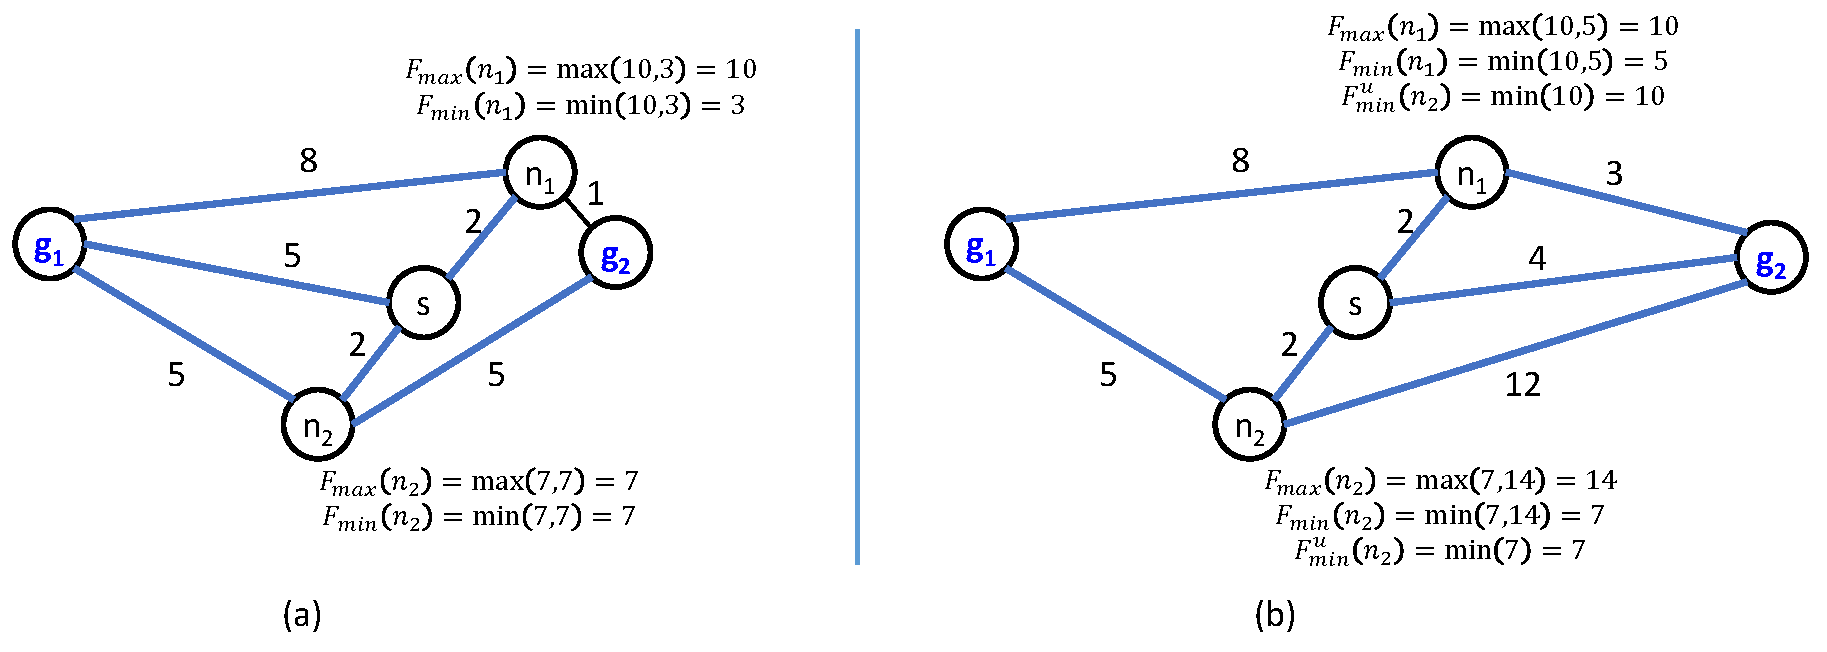
\includegraphics[width=\textwidth]{Lazy_cropped.pdf}
    \caption{The left hand graph shows an example where using Lazy \kastarmax{}
results in suboptimal solutions. The right hand graph shows a similar example,
but where using Lazy \kastarmin{} result in an optimal solution.}
    \label{fig:lazy}
\end{figure*}

\subsubsection{Lazy \kastarmin{}}

As an example, consider running Lazy \kastarmin{} on the graph depicted in the
right hand side of Figure~\ref{fig:lazy}. Assume we have a perfect heuristic in
all states except for the goal states $g_1$ and $g_2$ that have a zero
heuristic to each other, i.e., $h_2(g_1)=0$ and $h_1(g_2)=0$. After expanding
the start state $s$, states $n_1$, $n_2$, and $g_2$ are generated. Using
\minf{}, we have $F(n_1)=\min(10,5)=5$, $F(n_2)=\min(7,14)=7$, and
$F(g_2)=\min(0,0)=0$. So the next state expanded is goal $g_2$, which is then
removed from the set of active goals. At this stage, states $n_1$ and $n_2$ are
both in \open{} and their $F$ values are {\em stale}.
% in the sense that they were computed for $g_1$ and $g_2$ while the set of active goals at this stage contain only $g_2$ [[roni: already defined above]]
According to these stale $F$ values, the next state to
choose from \open{} is $n_1$ with $F(n_1)=5$. After popping $n_1$ out of
\open{}, however, its $F$-value is re-computed using Lazy \kastar{}. We denote
by $F^u_{min}(n)$ this updated $F$-value of $n$, which is computed with respect
to the current set of active goals. According to Lazy \kastar{}, if
$F^u_{min}(n)\geq F(n)$ then we set $F(n)$ to be $F^u_{min}(n)$ and re-insert
$n$ into \open{}. Consequently, $n_2$ will be expanded, followed by $g_1$,
finally finding the optimal path to $g_1$ as well.

We now prove that Lazy \kastarmin{} is correct for the general case.


% Lazy with minf is good
\begin{theorem}[Lazy \kastarmin{} is Equivalent to Eager \kastarmin{}]
Lazy \kastarmin{} expands exactly the same set of states as Eager \kastarmin{}, up to tie-breaking of states with the same $F$ value.
%Every path $\pi_i$ returned by Lazy \kastarmin{} is guaranteed to be the lowest-cost path to its corresponding goal ($g_i$).
\label{the:lazy-minf-correct}
\end{theorem}
\begin{proof}
We prove Theorem~\ref{the:lazy-minf-correct} by induction on the iterations
of Lazy \kastarmin{}, showing that Lazy \kastarmin{} and Eager \kastarmin{} expand exactly the same set of states.
The base of the induction is trivial: both Lazy and Eager \kastarmin{} expand the start state in the first iteration.
Now assume that in the first $m-1$ iterations both algorithms expanded the same set of states,
and consider the $m^{th}$ iteration of Lazy \kastarmin{}.

First, observe that for every state $n$ it holds that $F_{min}(n)\leq F^u_{min}(n)$, since $F^u_{min}(n)$ is the minimum over a subset of elements that $F_{min}(n)$ is a minimum of.
Now, let $n$ be the state expanded in the $m^{th}$ iteration of Lazy \kastarmin{}.
Since $n$ was chosen for expansion then it has the smallest $F$-value in \open{}.
In addition, its and $F$ value is not stale, as otherwise it
would have been re-inserted into \open{}. Thus, $F_{min}(n)=F^u_{min}(n)$.
Therefore
\[ \forall n'\in\open{} ~~ F^u_{min}(n)=F_{min}(n)\leq F_{min}(n') \leq F^u_{min}(n') \]
    So, $n$ has the smallest $F^u_{min}$ value in \open{}, and thus it would have also been expanded by Eager \kastarmin{}, as required.
\end{proof}
[[AF: The proof is hard to follow. We can talk and see. AF2: Sorry. I cannot
follow this proof]]
\roni{Improved it.}




% Lazy does not work for Max-f, but does work on Min-f
\subsubsection{Lazy \kastarmax{}}
Using Lazy \kastarmin{} has significant impact in practice, as it decides
in many cases to re-insert into \open{} the state with the minimal $F$ value. This is not the case in Lazy \kastarmax{}. In fact, Lazy \kastarmax{} will {\em never} re-insert a state into \open{} after re-computing its $F$ value.
This is because re-computing an $F$ value for a state after the set of relevant goals has been reduced will only cause the $F$ value to decrease. Thus, is a state already has the smallest $F$ value in \open{}, it will still have the smallest $F$ value after we re-compute its $F$ value.
Thus, for \kastarmax{} we only implemented the Eager approach.


\section{Theoretical Analysis}
\label{sec:theoretical-analysis}
% Analysis

In this section we compare analytically the two main approaches we proposed for
the \kgs{} problem: $k$ searches for one goal (\kxastar{}) or one search for
$k$-goals (\kastar{}).

\subsection{Expanded States and Memory Requirements}
First, we analyze the set of states expanded by the two approaches.
We denote by Exp(\astari{i}), Exp(\kxastar{}), Exp(\kastarmin), and Exp(\kastarmax),
the set of states expanded by \astari{i} (for a given $i$), \kxastar{}, \kastarmin, and \kastarmax{}, respectively. It is easy to see that
\[ Exp(\text{\kxastar{}})=\cup_{i=1}^k Exp(\text{\astari{i}}) \]

The relation between Exp(\kxastar{}), Exp(\kastarmin), and Exp(\kastarmax) is given in the following observation.
\begin{observation}
    \kastarmin{} expands exactly the same set of states as \kxastar{},
    and \kastarmax{} expands all these states and possibly more. Formally:
    \begin{enumerate}
        \item Exp(\kastarmin{})=Exp(\kxastar{})
        \item Exp(\kastarmax{})$\supseteq$ Exp(\kxastar{})
    \end{enumerate}
\label{obs:expandedStates}
\end{observation}
%\roni{Do we need a proof or is it trivial? AF: No, This is clear..}

% MAX not optimally effective
Note that there are cases where \kastarmax{} indeed expands surplus states,
i.e., cases where the set of states
expanded by \kastarmax{} is a strict superset of the set of states expanded by
\kxastar{}. For example, if there are two goals $g_1$ and $g_2$, and three
states in \open{} $A$, $B$, and $C$, such that ${\bf h}(A)=(2,9)$, ${\bf
h}(B)=(9,2)$, and ${\bf h}(C)=(5,5)$. The optimal path may be found without
expanding $C$, but using \kastarmax{} we will choose $C$ before $A$ and $B$.


% Memory=generated

The number of states expanded is directly related to the number of generated
states,\footnote{If $b$ is the branching factor then there are $b$ times more
    generated states than expanded states.} which in turn is related to the memory
requirements of \astar{} and \kastar{}. In general, best-first search
algorithms such as \astar{} and \kastar{} are memory intensive, storing the
states in \open{} and in \closed{} in order to be able to perform duplicate
detection and to choose the best state from \open{}. While other
implementations are also possible, where only the states in \open{} and their
predecessors are stored~\cite{zhou2006breadth,korf2004best} or where the states
are stored in external
memory~\cite{zhou2004structured,edelkamp2016external,edelkamp2005external}, we
focus our analysis on the more common implementation of \astar{} in which all
generated states are stored in-memory for the entire duration of the search.

Hence, the memory required for the algorithms discussed in this paper
proportional to the number of (distinct) states generated times the memory
required to store a single states.
%Without loss of generality, assume that each state requires one memory units to store and denote by Gen($X$) the set of states generated by algorithm $X$. From Observation~\ref{obs:expandedStates}, we can bound the memory required to run \kastarmin{} as follows:
In our analysis we make the simplifying assumption that each state requires one
memory unit to store for all algorithms. \footnote{This assumption is not
exactly correct in practice, since in \kastar{} we store for a state a vector
of $k$ values ($\textbf{f}(n)=(f_1,\ldots,f_k)$)  while in \astar{} we only
store a single value. Nonetheless, we justify our assumption for cases where
the memory required to store the state details is significantly larger than
these $k$ values.} Hence, if Mem($X$) and Gen($X$) denotes the memory required
and the of states generated when running algorithm $X$, respectively, then:
\begin{align}
Mem(\text{\kxastar{}})&=\max_{j\in [1,k]}| Gen(\text{\astari{j}})| \label{eq:kxastar-mem}\\
Mem(\text{\kastarmin{}})&=|\bigcup_{j\in [1,k]} Gen(\text{\astari{j}})| \label{eq:kastar-mem}\\
Mem(\text{\kxastar{}})&\leq Mem(\text{\kastarmin{}}) \leq \sum_{j\in[1,k]} Mem(\text{\astari{j}}) \label{eq:kxastar-kastar-mem}
\end{align}

The correctness of Equations~\ref{eq:kxastar-mem}-\ref{eq:kxastar-kastar-mem}
is now explained. Since \kxastar{} runs the $k$ searches individually, there is
no need to store the states generated by \astari{i} when running \astari{j}.
Thus, to run \kxastar{} we require memory sufficient to run each \astari{i}
individually (Equation~\ref{eq:kxastar-mem}). In \kastarmin{} we expand the
same set of states as \kxastar{} and thus generate the same set of states, but
we must store them throughout the search. Thus, \kastar{} stores every state
$n$ that is  generated by one of the $k$ searches in \kxastar{}, i.e., the
union $\bigcup_{j\in[1,k}Gen(\text{\astari{j}})$
(Equation~\ref{eq:kastar-mem}). The size of this union cannot be smaller than
the cardinality of the set of stated generated by any individual \astar{}, but
cannot be larger than their sum (Equations~\ref{eq:kxastar-kastar-mem}). Note
that these bounds are tight, in the sense that there are $k$-goal problems
where $Mem(\text{\kxastar{}}) = Mem(\text{\kastarmin{}})$ and other $k$-goal
problems where $Mem(\text{\kastarmin{}}) = \sum_{j\in[1,k]}
Mem(\text{\astari{j}})$.


\subsection{Runtime Analysis}

Now we analyze the expected runtime of the proposed \kgs{} algorithms. As shown
above theoretically and will be showed later experimentally, \kastarmin{} is
almost always superior to \kastarmax{}, and thus the focus of our analysis is a
comparison between \kxastar{} and \kastarmin{} (denoting the latter as simply \kastar{} throughout this section).  While both algorithms generate
the same set of states (Observation~\ref{obs:expandedStates}), their runtime
differ due to the number of times each state is generated and the cost of these
generations. Let Time($X$) be the running time required for algorithm $X$.
Computing Time(\kxastar{}) is straightforward: each one of the $k$ searches is
done independently, incurring a cost of $C_{gen}+C_{dd}+C_h+C_{add}$ per
generated state.
\[
Time(\text{\kxastar{}}) = \sum_{i\in[1,k]} |Gen(\text{\astari{i}})|\cdot (C_{gen}+C_{dd}+C_h+C_{add})
\]

For \kastar{}, a deeper analysis is needed. In addition to node generation ($C_{gen}$) and heuristic computation ($C_h$), in \kastar{} we also have the cost of re-sorting \open (either Eagerly or Lazily), which incurs $C_r$ for every state in \open{}.
Next, we consider the number of
times each of the costs components -- node generation ($C_{gen}$), heuristic computation ($C_h$), and state re-sorting ($C_r$) -- is incurred.

\noindent {\bf Node generation} ($C_{gen}$). Every generated state incurs
$C_{gen}$ exactly once. Thus, state generation add to the overall running time of \kastarmin{}:
\[
|\bigcup_{i\in{\{1,k\}}} Gen(\text{\astari{i}})|\cdot C_{gen} =
|Gen_k(\text{\kastar{}})|\cdot C_{gen}  \displaystyle
\]
\noindent {\bf Heuristic computation} ($C_{h}$).
Until the first goal is expanded, \kastar{} computes $k$ heuristics,
then, until the second is expanded, \kastar{} computes $k-1$ heuristics, and so on.
So, $Gen_k(1)$ states are generated with $k$ heuristics,
$Gen_{k}(2)$ states with $k-1$ heuristics,a nd so on. Summing all this, we have that
in \kastarmin{}, heuristic computations add to the overall running time:
\[ \sum_{i\in[1,k]} Gen_k(i)\cdot C_h \]


\noindent {\bf State re-sorting} ($C_r$).
\open{} gets re-sorted after every goal is found (except for the last goal).
The computational cost is the number of states in \open{} times $C_r$.
So, if $O_i$ is the number of states in \open{} when goal $g_i$ is expanded, then
the cost added to the overall running time that is due to adding states to \open{} is $\sum_{i\in[1,k-1]} O_i$.

\begin{table}
    \begin{tabular}{|l|l|l|}
        \hline
        Cost        & \kxastar{}                                    & \kastarmin \\ \hline
        $C_{gen}$   & $\sum_{i\in[1,k]} |Gen(\text{\astari{i}})|$       & * $|\bigcup_{i\in[1,k]} Gen(\text{\astari{i}})|$\\
        $C_{h}$     & * $\sum_{i\in[1,k]} |Gen(\text{\astari{i}})|$     & $\sum_{i\in[1,k]} |Gen_k(\text{\kastar{}})|$\\
        $C_r$       &   0                                               & $\sum_{i\in[1,k-1]} O_i$\\
        \hline
    \end{tabular}
       \caption{Analysis of the computational costs incurred by \kxastar{} and \kastarmin{}.}
       % when solving a \kgs{} problem with arbitrary $k$.  Some costs are incurred the same or less in one algorithm than the other. Such cases are marked with an asterisk.}
   \label{tab:time-analysis}
\end{table}


Table~\ref{tab:time-analysis} summarizes the above analysis, comparing the
running times of \kxastar{} and \kastarmin{}. Each row represents one of the
computational costs factors ($C_{gen}$, $C_{h}$, and $C_{r}$),
showing the contribution of that computational cost factor to the overall
running time for the compared algorithms. To show the usefulness of the above
analysis, we consider some special cases.
\begin{itemize}
    \item {\bf Case 1: State generation costs is dominant.} ($C_{gen}>>C_{h}+C_r$)
    If this case, the preferred algorithm is \kastar{}. To show this,
    compare the values in Table~\ref{tab:time-analysis} for $C_{gen}$: $\sum_{i\in[1,k]} |Gen(\text{\astari{i}})|$
    versus $|\bigcup_{i\in[1,k]} Gen(\text{\astari{i}})|$. Clearly, the former is larger than or equal to the latter.
    The advantage of \kastarmin{} grows with the size of the intersection between the sets $Gen(\text{\astari{i}})$ for $i\in[1,k]$.

    \item {\bf Case 2: Heuristic computation is dominant.} ($C_{h}>>C_{gen}+C_r$)
    If this is the case, the preferred algorithm is \kxastar{}. Again, to show this we look to Table~\ref{tab:time-analysis} and see that \kxastar{} computes a heuristic function
    $\sum_{i\in[1,k]} |Gen(\text{\astari{i}})|$ times, while
    \kastar{} computes the heuristic $\sum_{i\in[1,k]} |Gen_i(\text{\kastar})|$ times.
    Importantly, for every $i$ it holds that $|Gen_i(\text{\kastar})|\geq |Gen(\text{\astari{i}})|$
    because $Gen_i(\text{\kastar})$ contains all the states in $Gen(\text{\astari{i}})$
    and states from other searches that happen to have been added to \open{} at this stage.
\end{itemize}

\roni{Do we need the 2-goal illustration? I have text for it in the drafts.tex
[[AF: The two goal illustration will help a lot. I am for it. I almost started
doing it myself but if you have it, add it}
[[AF: This  $Gen_k(i)$ is a term that no one knows what it is. Can we
simplifies it]]
\roni{Revised. See if clearer}

[[Ariel up to here]]

\section{Experimental Results}

%In this section we compared empirically the performance of the four \kgs{} algorithms we discussed: $k$ \astar{} searches (Section~\ref{sec:k-one-goal}), two versions of \kastar{} (Section~\ref{sec:one-k-goal-search}): \kastarmax{} and \kastarmin{}, and Lazy \kastar{} with \minf{} (Section~\ref{sec:lazy}). We also compared these heuristic search algorithms with uniform cost search.

In this section we compared empirically the performance of the four \kgs{}
algorithms we discussed: \kxastar{} (Section~\ref{sec:k-one-goal}),
\kastarmax{} and \kastarmin{}(Section~\ref{sec:one-k-goal-search}), and Lazy
\kastarmin{}. A fifth algorithm is {\em uniform cost search} (UCS) (also known
as Dijkstra's algorithm) which is a best first search without a heuristic,
i.e., it prioritize nodes based on their $g$ values only.


We evaluated these algorithms on two domains: the pancake puzzle and path
finding in grids from the Dragon Age video game from the movingai
repository~\cite{sturtevant2012benchmarks}. These two domains represent
different types of search problems. The pancake puzzle is an {\em exponential
domain}, i.e., the state space graph is exponential in the size of the state,
and is given implicitly by a start state and a set of state transition
operators. The grid pathfinding domain is a {\em polynomial domain}, i.e., the
entire state space graph is given as input, and so the running time of a single
path finding search is polynomial in the problem input (the graph).

\roni{Meir, please add here details about the maps: which map did you use, etc.}
\subsection{Grid Path Finding}
\roni{Meir: what was the heuristic used? how were the states generated? how many instances?}

\begin{table}[]
    \centering
    \begin{tabular}{|r|r|r|r|r|r|}
    \hline
        & \multicolumn{1}{c|}{Lazy \kastarmin{}} & \kastarmax &      \kastarmin       &  \kxastar & UCS       \\

        \hline
1     & \textbf{1.9}                 & \textbf{1.9} & \textbf{1.9} & \textbf{1.9} & 3.5          \\
2     & \textbf{3.0}                 & 3.9          & \textbf{3.0} & 3.6          & 4.5          \\
4     & \textbf{4.0}                 & 5.7          & \textbf{4.0} & 6.9          & 5.2          \\
8     & \textbf{5.4}                 & 7.1          & 5.5          & 13.4         & 5.7          \\
16    & 7.0                          & 8.8          & 7.3          & 27.0         & \textbf{6.0} \\
32    & 9.1                          & 10.9         & 10.4         & 54.0         & \textbf{6.2} \\
64    & 12.5                         & 17.1         & 19.3         & 108.9        & \textbf{6.6} \\
128   & 20.5                         & 26.8         & 52.7         & 214.9 &
\textbf{6.7}\\
\hline
    \end{tabular}
    \caption{Running time (in ms.) spent when solving \kgs{} problems with different number of goals ($k$) on the grid pathfinding domain. Highlighted in bold are the best results for every $k$.}
    \label{tab:pathfinding-runtime}
\end{table}

In this domain we performed two type of experiments. In the first type of experiment, the goals were chosen randomly from the set of possible locations in the grid, and we investigated the impact of increasing the number of goals. The results are given in Table~\ref{tab:pathfinding-runtime}. The best results for every $k$ are highlighted in bold. There are several interesting trends to observe here. First, we clearly see that Lazy \kastarmin{} dominates both \kastarmin{} and \kastarmax{}. Second, we see that for every $k>1$, all version of \kastar{} outperforms \kxastar{}. Third, we see that as the number of goals becomes very large, UCS becomes the best algorithm. To explain this, consider the most extreme case, where we every state is a goal. In this case, clearly UCS will be the most effective, as it will expand every state at most once and will never spend any time on computing a heuristic value. By contrast, \astar{} and \kastar{} will compute at least one heuristic for every state, and most likely will compute even more heuristics per state. This heuristic computation time is not spent by UCS. Thus, as we see in the results the benefit of using a heuristic diminishes as the number of goals increase, resulting in UCS outperforming all other searches.



% Generated states.

\begin{table}[]
    \centering
    \begin{tabular}{|r|r|r|r|r|r|}
    \hline
        & \multicolumn{1}{c|}{Lazy \kastarmin{}} & \kastarmax &      \kastarmin       &  \kxastar & UCS       \\

        \hline
1                         & \textbf{13,987}                      & \textbf{13,987}           & \textbf{13,987}           & \textbf{13,987}                 & 41,122                      \\
2                         & 29,286                               & \textbf{21,682}           & 21,686                    & 27,389                          & 53,583                      \\
4                         & 43,291                               & \textbf{28,413}           & 28,424                    & 52,375                          & 62,826                      \\
8                         & 55,652                               & \textbf{36,650}           & 36,673                    & 101,103                         & 68,505                      \\
16                        & 64,805                               & \textbf{43,489}           & 43,531                    & 202,715                         & 72,196                      \\
32                        & 70,519                               & \textbf{49,662}           & 49,732                    & 407,221                         & 74,618                      \\
64                        & 73,841                               & \textbf{54,239}           & 54,357                    & 823,018                         & 75,998                      \\
128                       & 75,341                               & \textbf{57,739}           & 57,932                    & 1,613,628                       & 76,495\\
\hline
    \end{tabular}
    \caption{The number of states generated when solving \kgs{} problems with different number of goals ($k$) on the grid pathfinding domain. Highlighted in bold are the best results for every $k$.}
    \label{tab:pathfinding-generated}
\end{table}


%\begin{figure}
%   \includegraphics[width=0.45\columnwidth]{Capture-minf.PNG}
%   \includegraphics[width=0.45\columnwidth]{Capture-maxf.PNG}
%   \caption{XXx}
%   \label{fig:min-vs-max}
%\end{figure}

\begin{figure}
    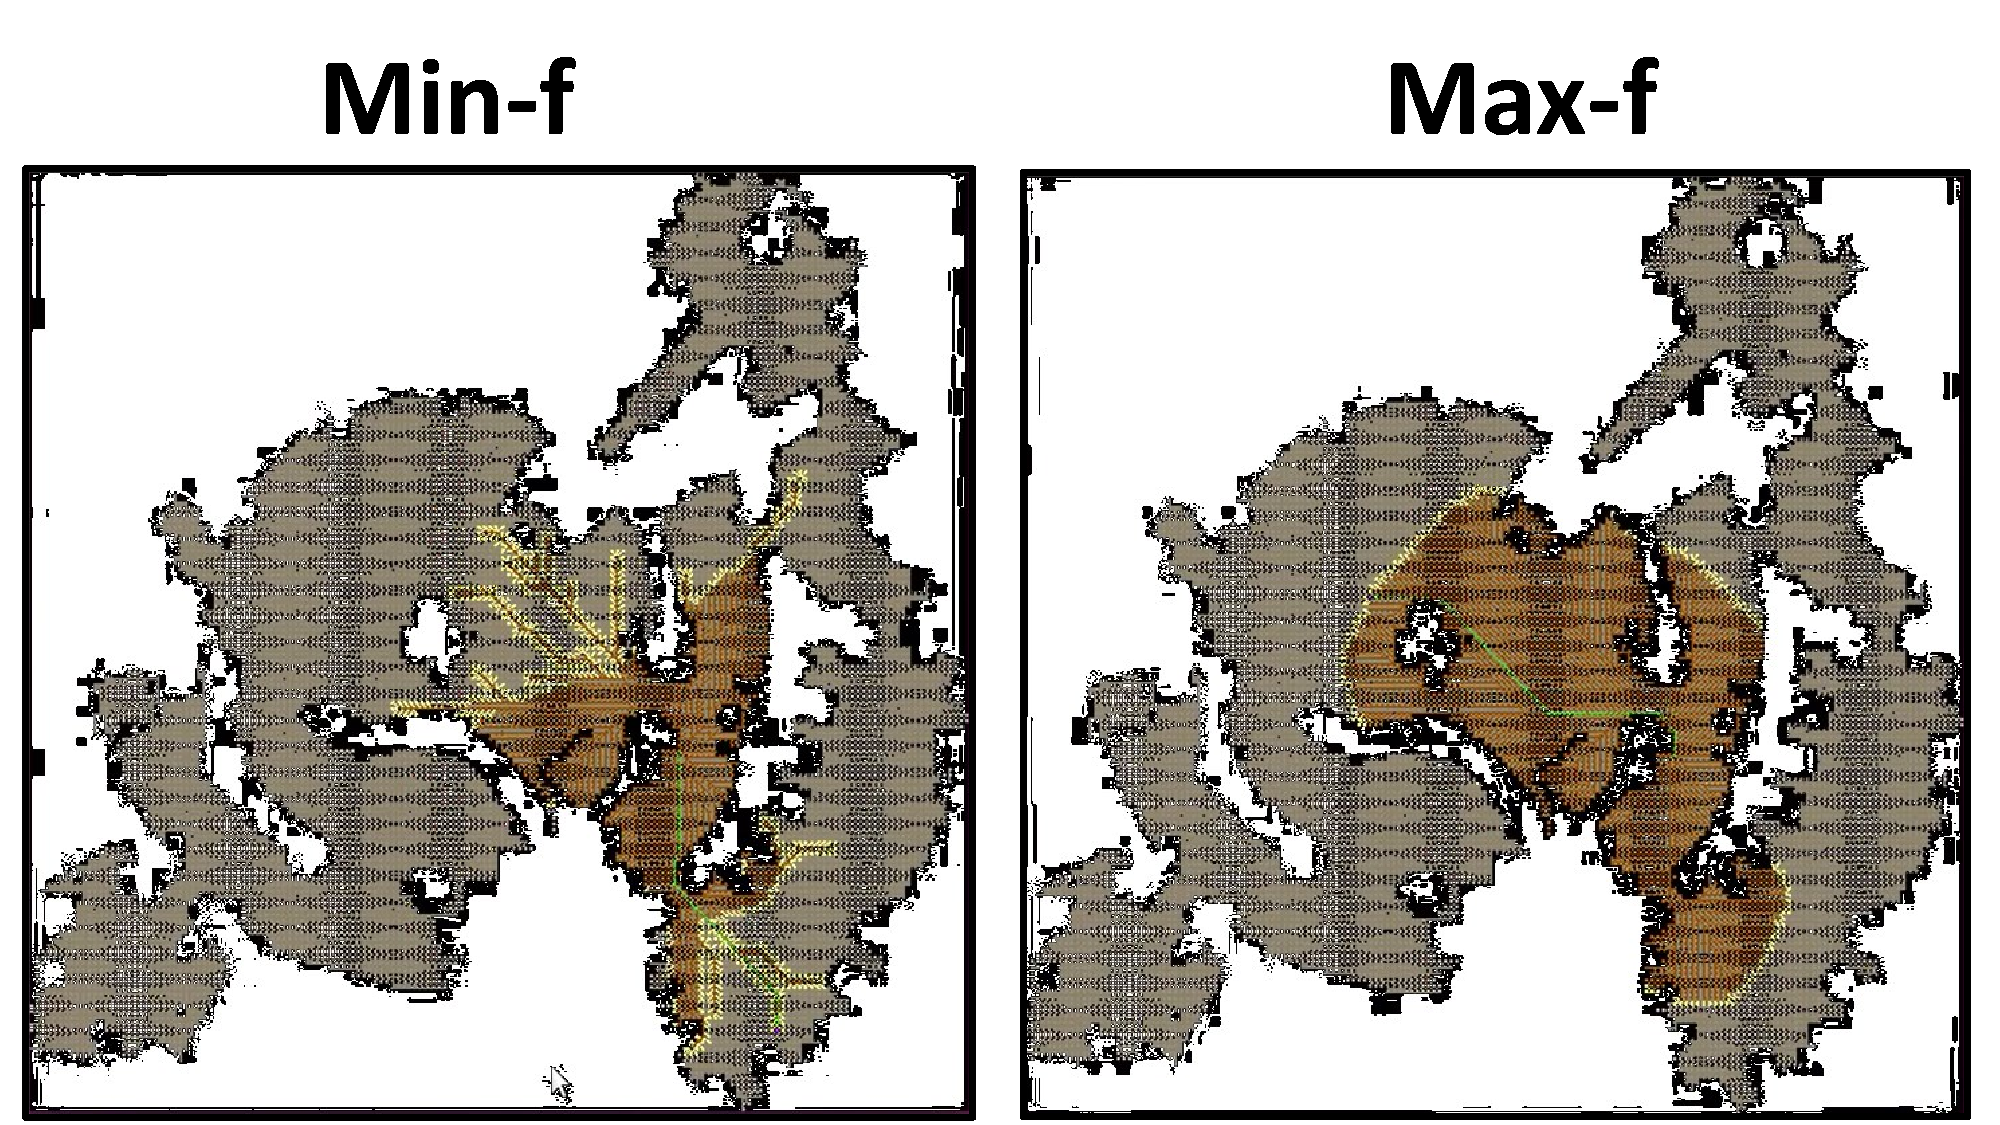
\includegraphics[width=\columnwidth]{min-vs-max}
    \caption{An example of running \kastarmin{} (left) and with \kastarmax{} (right). The yellow parts represent the states in \open{}, the brown parts represent the states in \closed{}.}
    \label{fig:min-vs-max}
\end{figure}

To provide a deeper insight, Table~\ref{tab:pathfinding-generated} shows the average number of states generated for each algorithm until it halts. Here too we highlihgted the best results for every $k$ in bold.
First, observe that even when the number of goals is large, uniform cost search generates more states than than the \kastar{} variants. This confirms our explanation above: when the number of goals is large, the  runtime of uniform cost search was lower than all other algorithm not because it generated fewer states, but because its time per state is smaller (due to not needing to compute heuristics).

Second, the number of states generated by \kastarmax{} is slightly smaller than that of \kastarmin{}. To explain this, consider the illustrations in Figure~\ref{fig:min-vs-max}. They show an example of running \kastarmin{} (left) and \kastarmax{} (right) on the same \kgs{} instance. The yellow points represent states in \open{}, the brown points represent states in \closed{}, the graph points are states that were not generated so far and the yellow points are impassable obstacles. As can be seen, the behavior of \kastarmin{} and \kastarmax{} are different: \kastarmin{} runs greedily towards prospective goals, showing clear trajectories protruding from the search frontier, while \kastarmax{} demonstrates a behavior that is more similar to uniform cost search. This is reasonable, because when in \kastarmin{} a child that is generated that is closer to the closest goal of its parent will expanded next, resulting in these protruding trajectories towards the goal. By contrast, in \kastarmax{} even if a state generates a child state that is closer to the closest goal, it still may not be expanded because it is further from some other goal. \roni{Probably there's a nicer way to explain this.}
[[AF: Yes there is. We need to think]]
This behavior results in \kastarmin{} having a weaker duplicate detection phase compared to \kastarmax{}, resulting in a bigger \open{} and thus more generated states.

\roni{Can anyone explain why Lazy \kastar{} generates more states?}
[[AF: Lazy should be identical to \kastarmin{}. Maybe they had different tie breaking?]]




\begin{figure}
    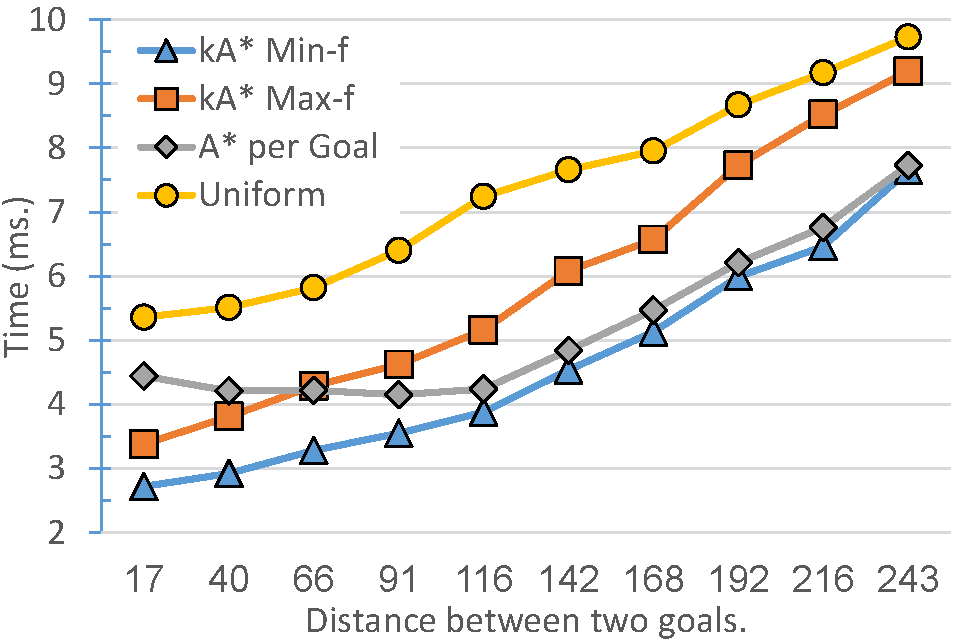
\includegraphics[width=\columnwidth]{G0-G1_cropped.pdf}
    \caption{This figure plots the runtime (in ms.) of the different \kgs{} algorithms as a function of the distance between the goals, for a \kgs{} problem with two goals ($k=2$).}
    \label{fig:2-goal}
\end{figure}
In the second type of experiments we performed, we focused on \kgs{} problems with two goals ($k=2$), and investigated the impact of the distance between these goals on the effectiveness of the evaluated algorithms.
The results are given in Figure~\ref{fig:2-goal}. The $x$-axis is the distance between the goals, and the $y$-axis shows the average runtime in milliseconds of the different algorithms.
\roni{Meir, is this Lazy \kastarmin{} or regular \kastarmin{}?}
We observe several trends.
First, for a 2 goal problem it is clear that uniform cost search is the worst option.
This is reasonable, as it does not use a heuristic to guide its search and the number of goals is small.
Second, observe that when the goals are close to each other, both \kastarmin{}
and \kastarmax{} outperform \kxastar{}. This matches our analytical analysis, where if the goals are close to each other we expect that there will be many states that will be expanded by both independent \astar{} searches, introducing exactly the redundancy \kastar{} was designed to solve.
Following this explanation, we observe that as the goals chosen become further from each other (going right on the $x$ axis of Figure~\ref{fig:2-goal}), we see the advantage of \kastar{} over 2 \astar{} searches diminishes. Indeed, the performance of \kastarmin{}  and \kxastar{} converge when the goals are furthest from each other.
Lastly, we observe that \kastarmin{} dominates \kastarmax{} and in general all other approaches, always being better or on par with the other algorithms.

\subsubsection{Impact of Using Stronger Heuristics}

\begin{figure*}
	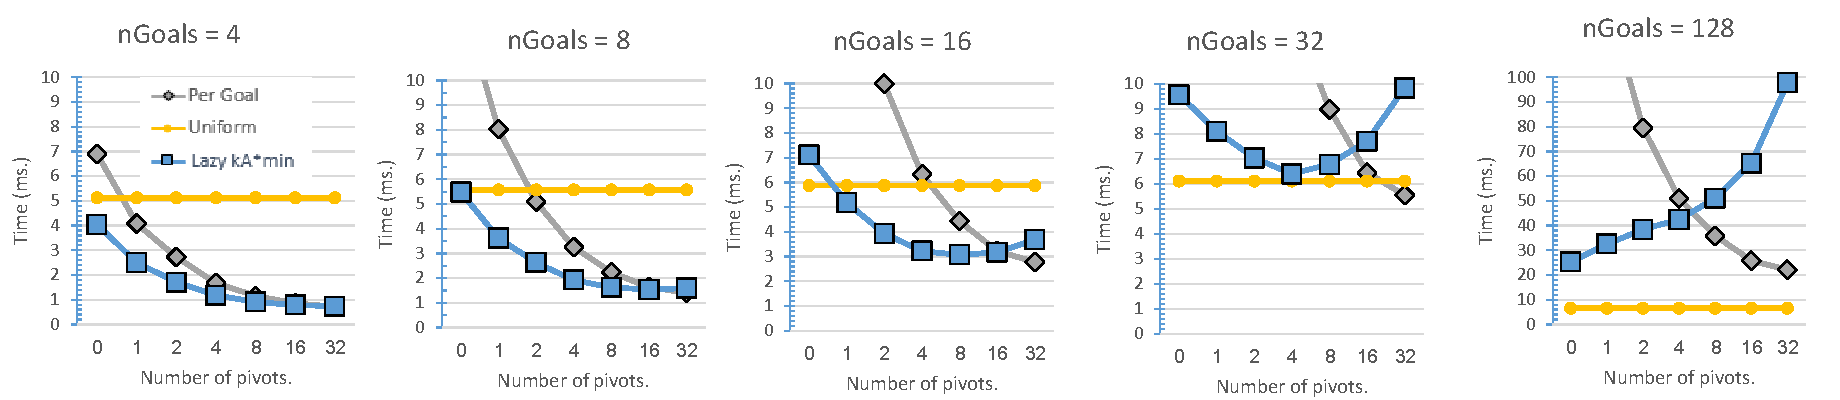
\includegraphics[width=\textwidth]{heuristic-power_cropped.pdf}
	\caption{The running time of Lazy \kastarmin{}, \kxastar{}, and UCS for different number of goals (the different plots) and difference number of pivots using in the heuristic computation. The heuristic is more accurate but slower to compute.}
	\label{fig:dh-results}
\end{figure*}

Next, we evaluated the impact of using a stronger, i.e., more accurate, heuristic, on the performance of the proposed \kgs{} algorithms. To this end, we used differential heuristics (DH)~\cite{who}, a state-of-the-art heuristic for grid pathfinding. In DH, a set of states (cells in the grid) are chosen upfront and the all pairs shortest paths are pre-computed. Then, when computing the heuristic for a state that is not part of these states, 
one can use the triangle inquality to obtain an admissible heuristic. 
Importantly, adding more pivots results in a more accurate heuristic, 
but one that takes longer time to compute. 

Thus, DH is especially useful for our analysis, as it can be tuned to more accurate and more costly to compute. The results of Lazy \kastarmin{}, \kxastar{} and UCS are given in Figure~\ref{fig:dh-results}. Each of the 5 plots show the average runtime in milliseconds on the $y$ axis, and the $x$ axis shows the number of pivots used for computing the heuristic. 
The different plots show the results for 4, 8, 16, 32, 64, and 128 goals. 
As expected, the running time of UCS is unaffected by the number of pivots, since it does not use a heuristic. Also, we observe that as the number of goals increase, the benefit of using heuristic search over plain UCS diminishes. Eventually, when solving for 128 goals, UCS dominates both \kastarmin{} and \kxastar{}. %solving for large number of goals eventually 

Next, consider the impact of adding pivots -- i.e., using a stronger but more costly heuristic. 
For the \kxastar{}, we observe that adding pivots always helps reducing running time. For \kastarmin{}, however, adding pivots improves running time only for cases when the number of goals was not very large. For example, when $k=32$, using more than 4 pivots actually degrades the performance of \kastarmin{}. These results conform with out theoretical analysis: adding pivots increase $C_h$, which is incurred more times in \kastarmin{} than in \kxastar{}. 

%This is done  \kastar{} and \kxastar{} in 


\subsection{Pancake Puzzle}

\begin{table}[]
    \centering
    \begin{tabular}{|r|r|r|r|r|}
    \hline
        \multicolumn{1}{|l|}{}            & \multicolumn{2}{c|}{Runtime (ms.)}                                       & \multicolumn{2}{c|}{Generated} \\ \hline
        \multicolumn{1}{|c|}{\# Pancakes} & \multicolumn{1}{c}{\kastarmax{}} & \multicolumn{1}{c|}{Uniform} & \multicolumn{1}{c}{\kastarmax{}} & \multicolumn{1}{c|}{Uniform} \\ \hline
        6                               & 0.34                                      & 0.46                        & 994                                       & 2,287                       \\
        7                               & 2.57                                      & 4.06                        & 8,617                                     & 21,059                      \\
        8                               & 22.95                                     & 40.25                       & 74,745                                    & 188,946                     \\
        9                               & 410.81                                    & 717.64                      & 787,481                                   &
        1,973,420\\
        \hline
    \end{tabular}
    \caption{Running time (in ms.) and number of generated states for solving \kgs{} with two goals
        in the Pancake puzzle domain using UCS and \kastarmax{}.}
\label{tab:pancake-max-uniform}
\end{table}

Next, we present the results for the pancake puzzle.
\roni{Meir: what was the heuristic used? how were the states generated? how many instances?}
The first results we report is that uniform cost search and \kastarmax{}
could not solve even small-sized problems even for $k=2$. Average running time and number of states generated  for $k=2$ and pancakes of size up to 9 are given in Table~\ref{tab:pancake-max-uniform}. These results are reasonable because in exponential domains running a search without a heuristic is not practical, and \kastarmax{} can behave similar to uniform cost search (as shown also in Figure~\ref{fig:min-vs-max}).


\begin{table*}[]


            \centering
        \begin{tabular}{|r|r|r|r|r|r|r|r|r|}
            \hline
            & \multicolumn{4}{c|}{{\bf 10 Pancakes}} & \multicolumn{4}{c|}{{\bf 20 Pancakes}}    \\
            \hline
            & \multicolumn{2}{c|}{Average of Time (ms.)}   & \multicolumn{2}{c|}{Average of Generated}    & \multicolumn{2}{c|}{Average of Time (ms.)}   & \multicolumn{2}{c|}{Average of Generated}    \\
            \hline
            $k$ & \kastarmin{} & \kxastar{} & \kastarmin{} & \kxastar{} & \kastarmin{} & \kxastar{} & \kastarmin{} & \kxastar{}  \\ \hline

1           & 0.09                  & \textbf{0.08}       & \textbf{190}          & \textbf{190}        & 4.24                  & \textbf{4.17}       & \textbf{7,324}        & \textbf{7,324}      \\
2           & 0.20                  & \textbf{0.16}       & \textbf{363}          & 368                 & 9.75                  & \textbf{7.81}       & \textbf{13,794}       & 13,828              \\
4           & 0.51                  & \textbf{0.35}       & \textbf{755}          & 788                 & 21.74                 & \textbf{13.73}      & 25,154                & \textbf{24,982}     \\
8           & 1.18                  & \textbf{0.67}       & \textbf{1,364}        & 1,512               & 66.63                 & \textbf{30.14}      & \textbf{53,268}       & 53,790              \\
16          & 3.24                  & \textbf{1.35}       & \textbf{2,645}        & 3,058               & 206.03                & \textbf{59.51}      & \textbf{103,674}       & 105,863     \\ \hline
    \end{tabular}
    \caption{The average runtime and average number of states generated in the pancake experiments, for \kastar{} with \minf{} and for running $k$ independent \astar{} searches. Best results per $k$ are highlighted in bold.}
    \label{tab:pancake-minf-k-searches}
  \end{table*}


Table~\ref{tab:pancake-minf-k-searches} presents the results for 10 pancakes and for 20 pancakes, for 1, 2, 4, 8, and 16 goals, comparing \kastarmin{} and \kxastar{}.
The results show that while \kastarmin{} usually generates fewer states, its overall runtime is comparable or worse than running \kxastar{}. This is because in exponential domains the intersection between the sets of states generated by each search is small compared to size of the last $f$ layer of each search. \roni{Meir and Ariel, I'm looking for a nicer explanation. Any thoughts?}


\begin{figure}
    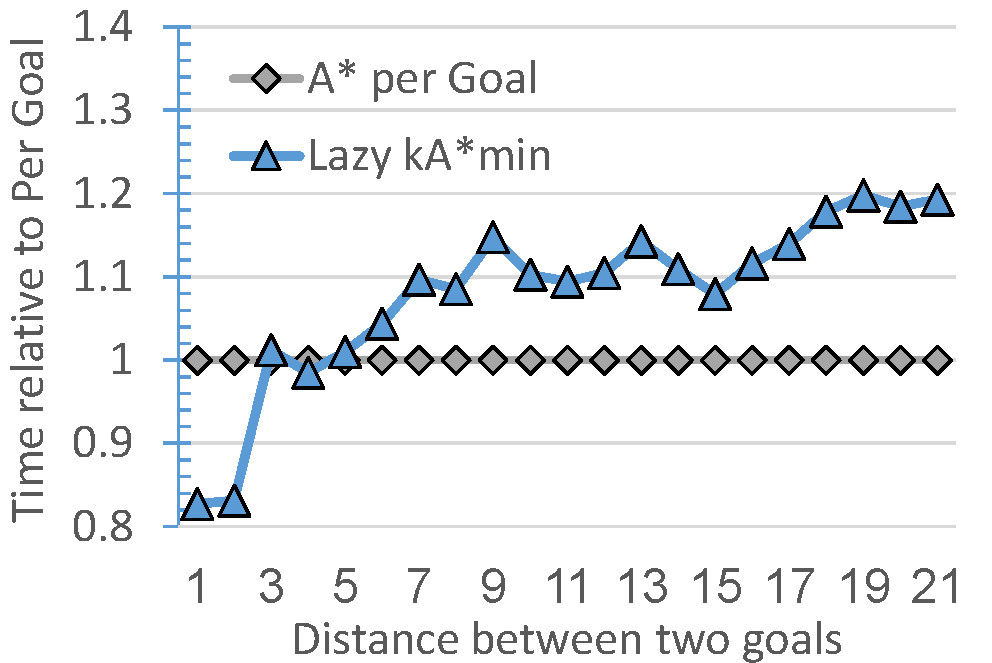
\includegraphics[width=\columnwidth]{pancake-goal-distance_cropped.pdf}
    \caption{10 pancake domain. Runtime as a function of the distance between the goals in \kgs{} with two goals.}
    \label{fig:2-goal-pancake}
\end{figure}


To gain a deeper insight into the behavior of the various \kgs{} algorithm in this domain, we performed additional experiments.  Figure~\ref{fig:2-goal-pancake} plots the running time of Lazy \kastarmin{} and \kxastar{} for a \kgs{} instance with two goals ($k=2$). Here, we show the relative running time of \kastarmin{} compared to \kxastar{}. Similar to Figure~\ref{fig:2-goal}, the $x$-axis here is the distance between the goals. We generate problem instances for this experiment by choosing the standard goal state (where all pancakes are ordered nicely) and performing and limited number of random walks from it. We compared the performance of \kxastar{} and Lazy \kastarmin{} for \kgs{} problems with two goals, where we varied the distance between the two goals. This was done by choosing the second goal by performing a limited number of random walks.


As we observed in the grid path finding domain, when the goals are very close, \kastarmin{} is better, as there is a large intersection between the states generated when searching both goals. However, we observe here that unlike the grid path finding domain, the advantage of \kastarmin{} quickly disappears, and for cases where the goals are more than 5 steps apart it is better to use \kxastar{}. This supports are analysis, as in exponential domains a small distance between the goal can result in needing a very large number of unique states to expand per goal.



To conclude our experimental results, we observed the following trends:
\begin{enumerate}
    \item In the pancake domain, running $k$ individual searches (\kxastar{}) is better than \kastar{}, because the overlap of states generated by more than one search is small.
    \item In the grid pathfinding domain, however, many states are generated by more than one search, and consequently \kastar{} is advantageous compared to \kxastar{} searches.
    \item \kastarmin{} usually outperforms \kastarmax{}, but not always. Lazy \kastar{} outperforms both.
    \item When the number of goals becomes very large, simply running UCS is the best option, as it does not spend time on heuristic computations.
\end{enumerate}

\roni{TODO: ADD MORE HERE}




\subsection{Related work}
\label{sec:related-work}

\kgs{} is similar to many previously studied problems. As mentioned in the introduction, it is different from TSP in that in TSP the task is to find a shortest path that passes through a set of vertices, while in \kgs{} that task is to find $k$ shortest path, one to each vertex. In that sense it is similar to the minimal spanning tree (MST) problem, but we only require optimal path to a selected set of $k$ vertices and not to all vertices (as in MST).


\kgs{} is also different from a disjunction of $k$ goals, i.e., from the case where there are $k$ possible goals and the task is to find the lowest cost path to the closest one. Unlike this case of a disjunction of $k$ goals, in \kgs\ we must find the shortest path to each of the goals, and not just to the closest one.

Somewhat related is the work on {\em multi-objective search}, where we have multiple objectives function that we wish to optimize. For example, in a navigation application one may want to optimize for path length and also for ease of navigation. An optimal solution to a multi-objective optimization problem is usually a solution that is Pareto-optimal, and it is often the case that one would like the set of all Pareto-optimal solutions. This is fundamentally different from \kgs{}, where we have a single optimization criteria -- we must have the lowest-cost path to all $k$ goals.


The \kgs{} problem is related to the problem addressed by incremental search algorithms such as Lifelong Planning \astar{}~\cite{koenig2004lifelong},  D*-Lite~\cite{koenig2005fast}, and Path-Adaptive A*~\cite{hernandez2015reusing}. Incremental search algorithm are designed to solve a sequence of search problems, where the start and goal of these search problems are the same, but the underlying graph has changed. The key idea in incremental search algorithms is to re-use information from previous searches to solve faster the current search problem. However, unlike the incremental search setting is different from \kgs{}: in incremental search we have one goal and the environment is dynamic, while in \kgs{} we have $k$ goals but assume the environment does not change.

Another related problem is the moving-target search problem~\cite{koenig2007speeding,ishida1991moving}. Moving-target search problems are search problems where the goal changes during the search. This is different from \kgs{} where the goals do not change during the search, but we know upfront the $k$ goals.


\section{Conclusion and Future Work}
In this work we studied the \kgs{} problem, and analyzed two fundamental approaches for solving it: $k$ single-goal searches and a single search for $k$ goals. We analyzed the deficiencies of $k$ single-goal searches and formalized \kastar{}, a single algorithm that searches for $k$ goals together.
Three variants of \kastar{} were presented: \kastarmax{}, Eager \kastarmin{}, and Lazy \kastarmin{}. Given an admissible heuristic, both Eager and Lazy \kastarmin{} are sound and complete, and if the heuristic is consistent so is \kastarmax{}. We then analyzed all the proposed algorithms theoretically, comparing their memory requirements and running time. Finally, we performed an experimental study on two domains, showing that empirically Lazy \kastarmin{} dominates the other \kastar{} variants. In addition, our results suggest that
in polynomial domains it is usually the case that running \kastar{} is better than running $k$ individual \astar{} searches, but in exponential domains running $k$ individual searches is usually better. In addition, if the number of goals is very large then running uniform cost search may be the best option.


This work is, to the best of our knowledge, the first study of using heuristic search techniques to solve \kgs{}. There are several exciting directions for future work. First, we only explored in this work how to avoid some of the redundant computations done when performing $k$ individual searches. As mentioned briefly in Section~\ref{sec:k-one-goal}, a different way to benefit from searching for multiple goals is that while searching for one goal one can learn valuable information about the underlying graph, which may later be used to improve the search. This can include, for example, learning techniques to improve the quality of the heuristic.

One way to do so in undirected graphs is to use the heuristic for one goal and the heuristic between the goals as an admissible heuristic, thus allowing to save the computational cost of re-computing the heuristic of a state if it is generated again for the other goal. This idea is inspired from memory-based heuristics used by path finding algorithms~\cite{sturtevant2007memory,sturtevant2009memory,goldenberg2011theCompressed}.

Another way to learn information about the search space is to compile \kgs{} to an incremental search problem. This can be done by adding an artificial vertex that is connected to all goals, and running the search from this goal to the start state. Then, every iteration of the incremental search algorithm will change the weight of the edges from the artificial goal to the actual goal, setting the edge to exactly one goal with zero weight and all other edges as unpassable. This compilation may enable using incremental search algorithm such as Path-Adaptive A*~\cite{hernandez2015reusing} to solve the \kgs{} problem.





% \begin{figure}[!htbp]
%   \centering
%   \includegraphics[width=1\hsize]{filename.eps}
%   \caption{caption} \label{fig:label}
% \end{figure}

\section*{Acknowledgements}
Thanks!

\bibliographystyle{abbrv}
\bibliography{library}

\end{document}
